\chapter{基础数据交换的需求分析与概要设计}
\section{全动飞行模拟机整体概述}
现代的飞行模拟机由模拟座舱、仿真机、视景系统、声音系统、运动系统等构成。其运作方式如图\ref{simstruct}所示。模拟座舱是一比一还原的对应型号飞机驾驶舱,飞行员通过操作各种操作杆与按钮驾驶飞机。
这些操作会作为核心组件仿真机的输入,经过仿真计算后得到一系列的状态,比如当前飞机所处的位置,飞行的姿态,以及环境声音等等。教练员也可以增加如雨雪天气之类的设定,实现不同场景下的训练。
这些状态会以指令的形式给到各个系统,视景系统根据指令完成场景搭建和画面渲染,声音系统据此产生各类音效,运动系统据此调整模拟座舱的姿态或产生体感加速度。
\begin{figure}[h]
    \begin{center}
        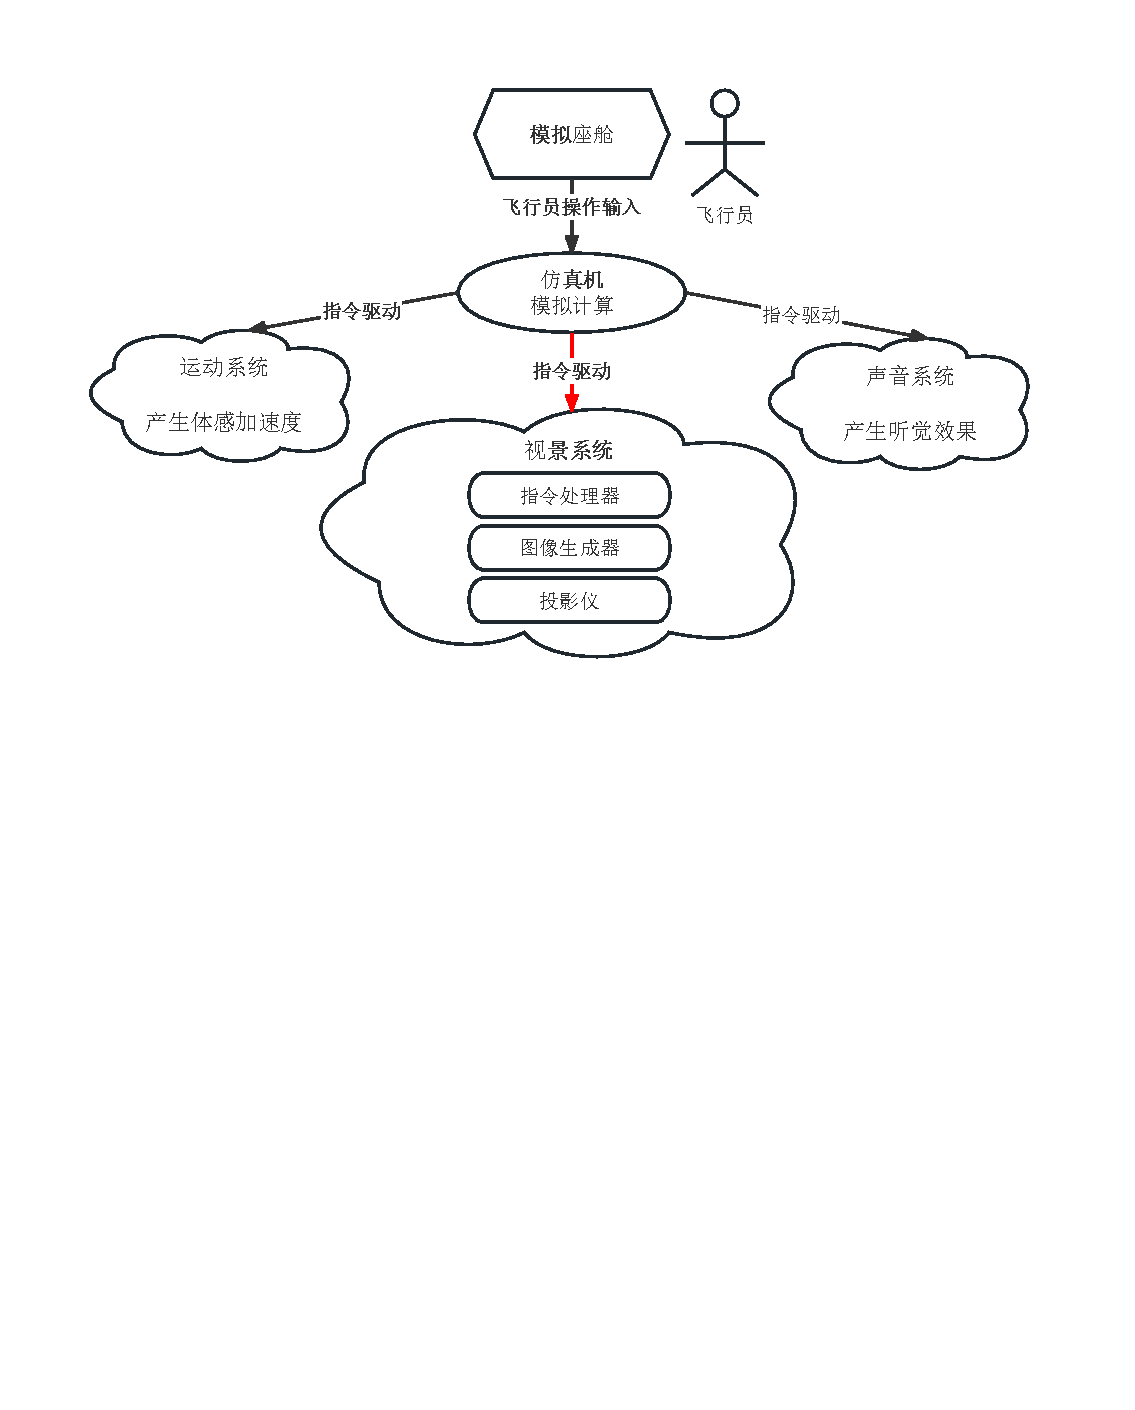
\includegraphics[width=.9\textwidth]{pictures/simstruct.pdf}
        \caption{模拟机运转方式}
        \label{simstruct}
    \end{center}
\end{figure}
\par
由上述可知仿真机相当于整个FFS的服务端,所有系统都需要与其连接,听从指令才能正常工作。
因此,想要基于现有仿真机开发视景系统,首先要理解该仿真机输出的指令,包括其中的数据组织结构和数字表示方法等。
\section{仿真机数据帧分析}
\subsection{数据帧的获取}
对于仿真机与视景系统间行为的分析,最直接的想法是获取处理指令的源代码。经过一番探索,在其中发现了名为Visual Interface进程。但该程序是编译型语言最终得出的二进制指令,并不知道其使用怎样的编译器编译而来;而且此方式通常用于分析主干代码,并不适合获取我们需要的指令细节,这是一条时间成本与预期结果都无法估算的路径。
幸运的是,我们同时拥有一份关于该仿真机的文档,其中含有对于仿真机与视景系统交互指令的详细说明,唯一的问题是该文档编写于20多年前,其时效性有待验证。
\par
有了以上思路后,关于仿真机指令的分析方法就从获取源码变为了验证文档。对于两方通讯方式的研究,网络流量分析也是重要的方法。
为了验证文档内容的正确性,我们使用网络抓包工具WireShark截取了运行时仿真机与视景系统交流的原始数据帧,验证数据帧的组织结构与数字表示方法是否与文档中的说明相符。
图\ref{datastruct}为文档中定义的数据帧结构,也就是说在理想情况下我们可以对捕获的数据帧按照该结构进行拆分。
\begin{figure}[h!]
    \begin{center}
        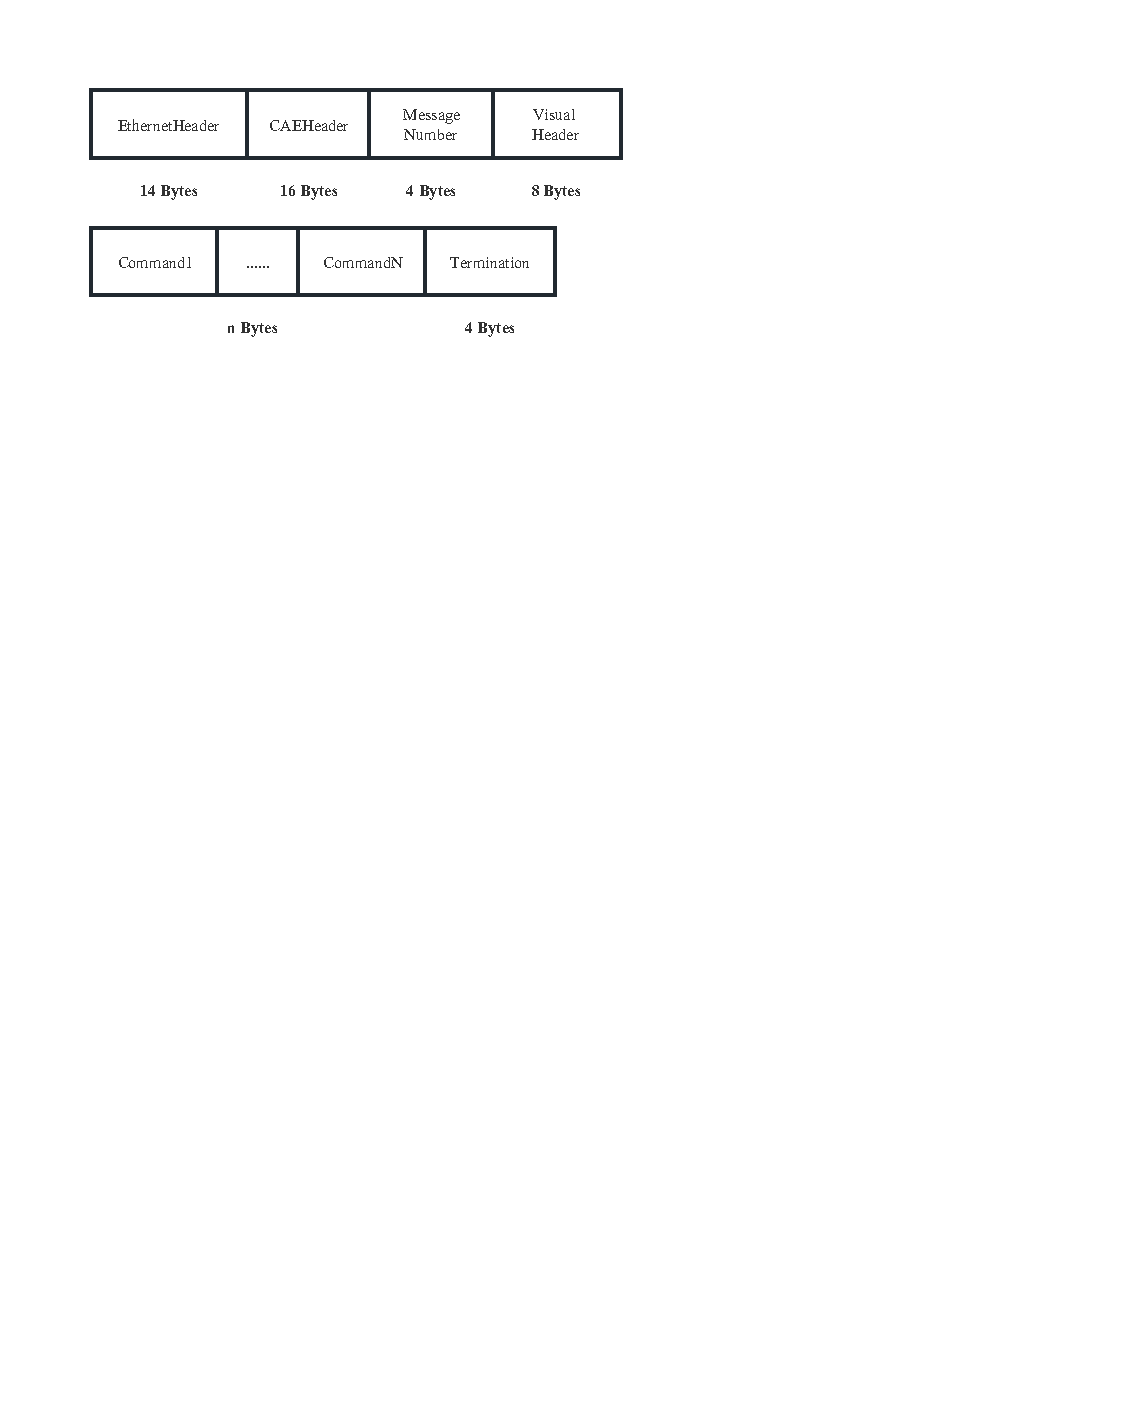
\includegraphics[width=.8\textwidth]{pictures/datastruct.pdf}
        \caption{CAE仿真机数据帧结构}
        \label{datastruct}
    \end{center}
\end{figure}
\par
在上述结构中我们最需要关注的是指令Command的具体结构。文档中关于指令结构的定义如图\ref{commstruct}所示。
指令的数据部分前有8字节的头部信息,目前来说比较重要的头部信息一是Opcode,它是每一种指令的代号,是指令的身份证。我们可以通过代号得知指令Data部分的组织结构,以此来进行反序列化。
第二是Size,它表明了这条指令的总长度,此信息可以帮助拆分数据帧中的多条指令。

\begin{figure}[h!]
    \begin{center}
        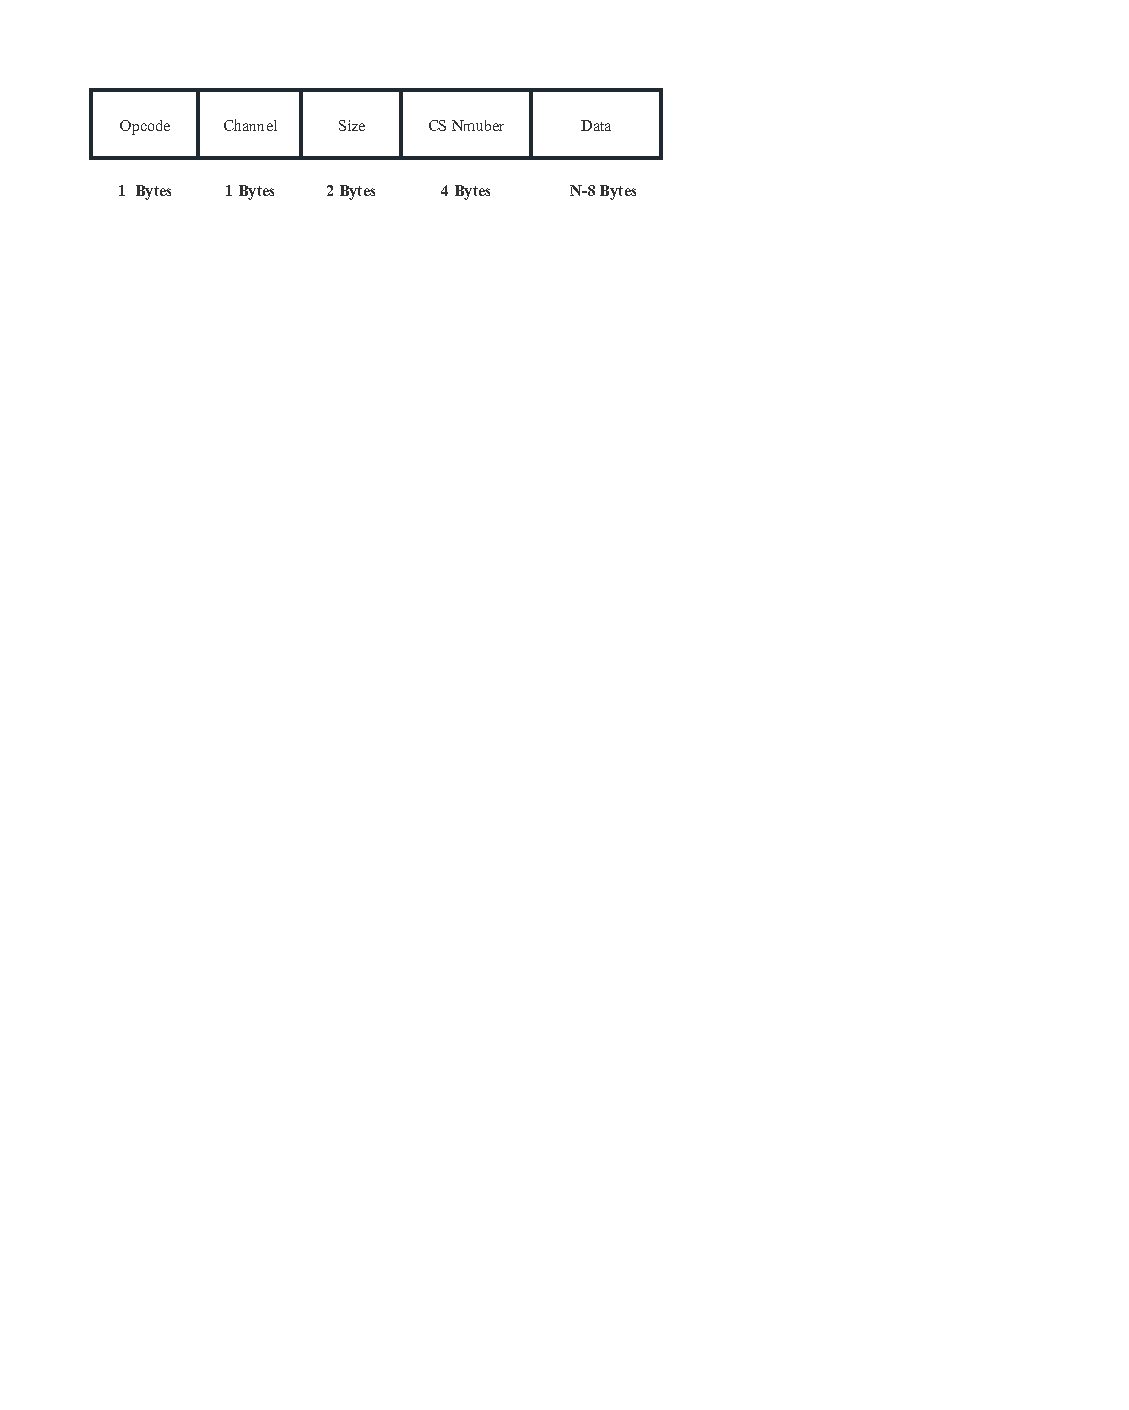
\includegraphics[width=.8\textwidth]{pictures/commStruct.pdf}
        \caption{数据帧中的指令结构}
        \label{commstruct}
    \end{center}
\end{figure}
\par
图\ref{framedata}展示了通过WireShark捕获到的流经视景系统网卡的一个数据帧。
最左侧一列是对字节的计数,为十六进制,该数据帧共有90字节。依照文档中仿真机数据帧结构来看,
第一行前14字节为以太网协议头,分别表示源mac地址,目标mac地址和除去该协议头后的长度,004c正好表示76字节。
跳过所有头部信息来到指令部分,第三行的86表示这之后是代号为86的指令数据段。以此来看,文档中对于数据帧结构的描述是正确的。
\begin{figure}[h!]
    \begin{center}
        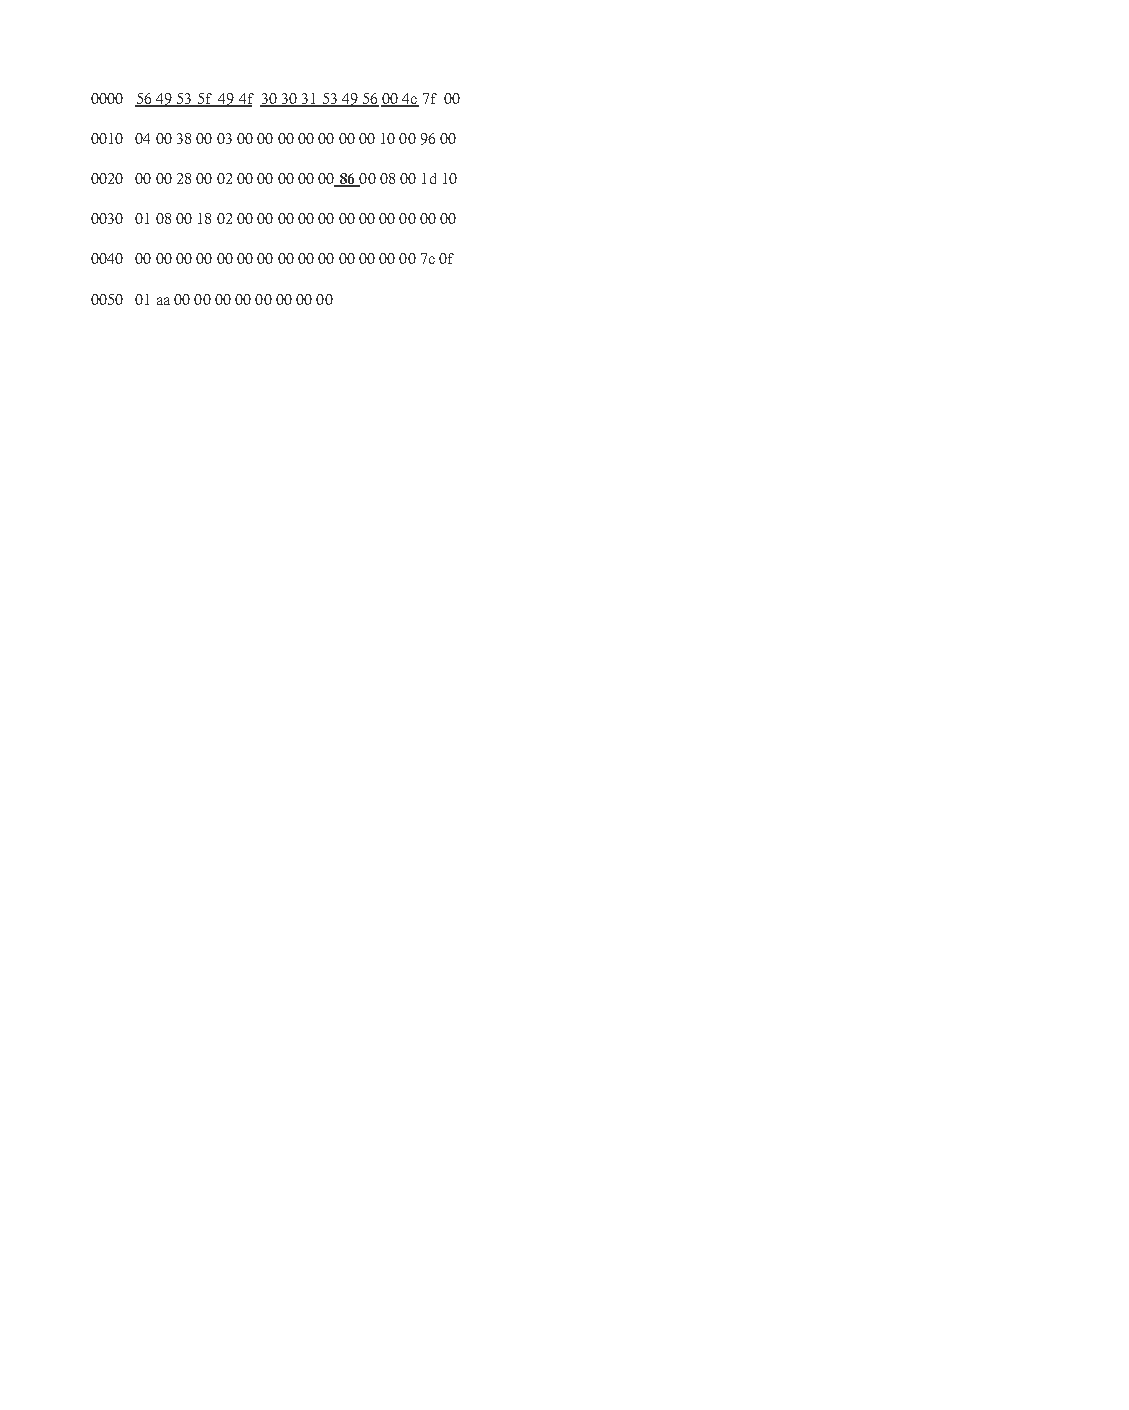
\includegraphics[width=0.7\textwidth]{pictures/framedata.pdf}
        \caption{捕获的数据帧}
        \label{framedata}
    \end{center}
\end{figure}
\subsection{数据帧的解读}
通过对比文档中的数据帧结构说明和截取到的真实数据帧,从该数据帧头部仅有Ethernet Header可以得出仿真机网络协议栈非常简单。从网络模型角度看其最高层是数据链路层,数据内容用以太网协议封装后便进行发送,接收数据也只能仅被以太网协议封装过,否则仿真机无法正确理解反馈信息。因此无法通过工作于传输层以上的传统socket连接模式与本视景系统交流。
图\ref{netlayer}形象的解释了仿真机与视景系统的网络层级差异。
\begin{figure}[h]
    \begin{center}
        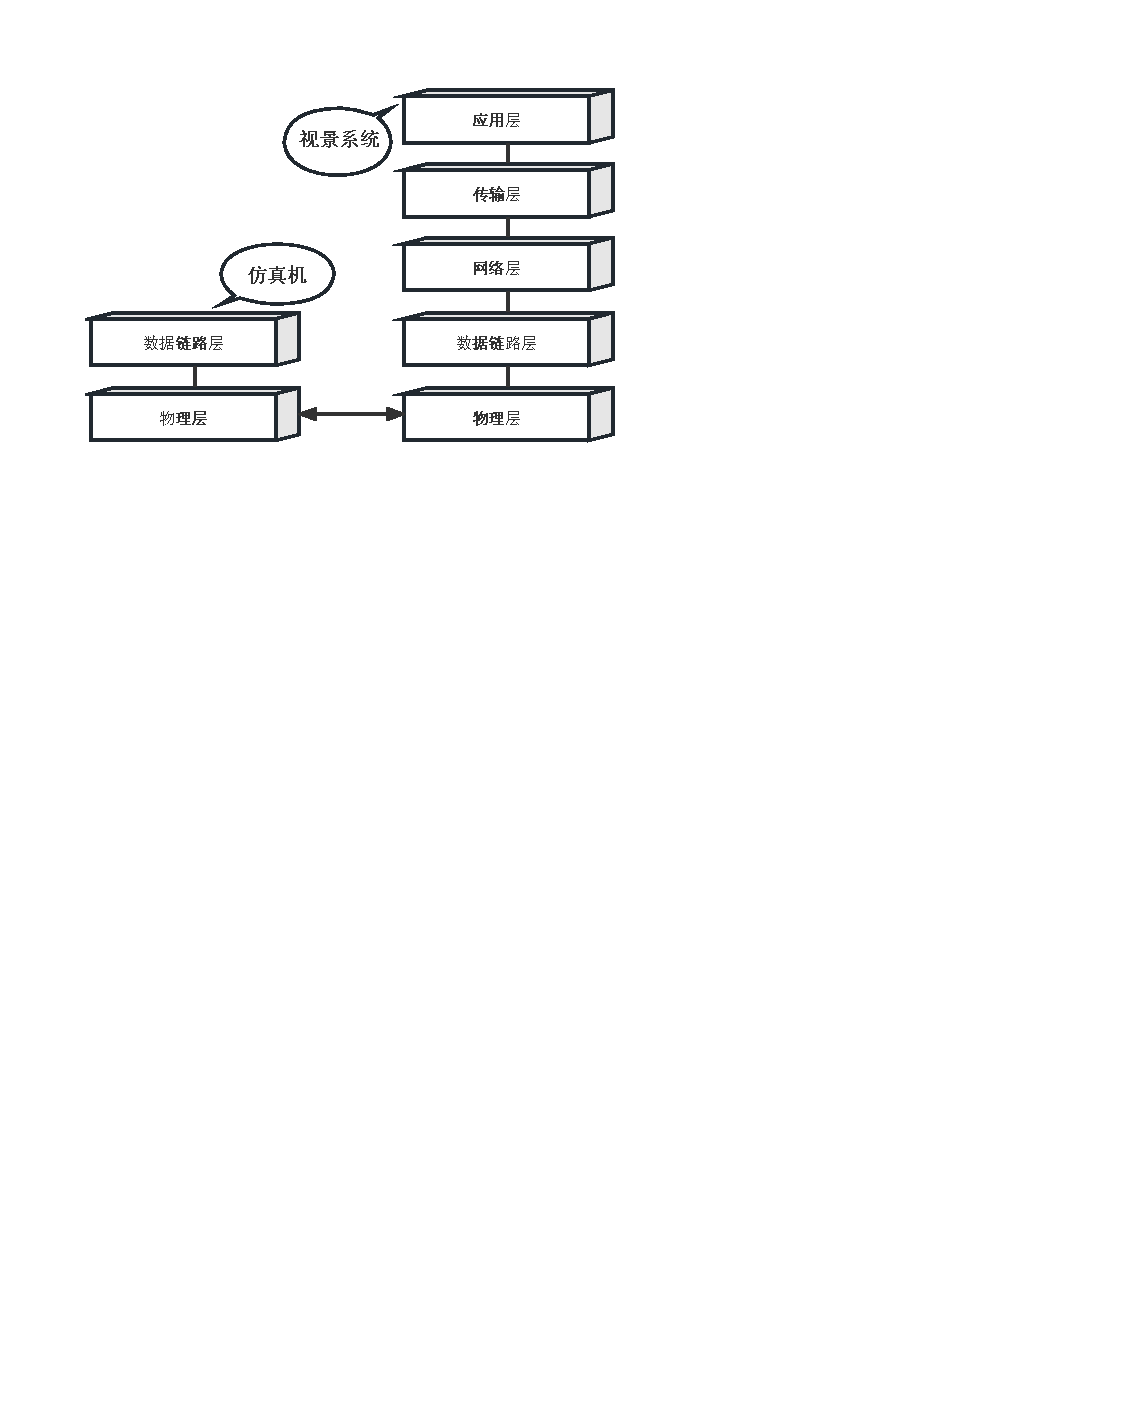
\includegraphics[width=.8\textwidth]{pictures/netlayer.pdf}
        \caption{仿真机与视景系统层级差异}
        \label{netlayer}
    \end{center}
\end{figure}
\par
当剥去数据帧头部的以太网协议头和CAE自定义的部分信息后便余下该数据帧中的所有指令数据,一个数据帧可能包含多条指令。
此处以指令代号为21H(H表示十六进制)的指令为例,此指令在飞行模拟中十分关键,其中以经纬度海拔和欧拉角的形式给出了飞机的位置和姿态信息,是仿真机每帧运行都要发出的指令。
文档中关于该指令数据结构的描述如图\ref{21h}中的结构体所示。其种Int32仅代表对应字段占据了32bit,并不表示实际数据类型。由于仿真机侧的数据序列化并没有使用任何数据交换协议,
如果文档内容正确,则可以直接使用该结构体完成对应数据段的反序列化。
\begin{figure}[h!]
    \centering
     \lstinputlisting[basicstyle= \zihao{-5}]{pictures/21h.txt}
    \caption{21H指令结构}
    \label{21h}
\end{figure}
\par
为了验证文档的时效性,我们需要对该指令中数据的合理性进行检查。在这步工作前需要先进行数字表示方式的转换。
仿真机发送指令中的字段并不是可以直接读取的浮点数,需要做出进一步的转换。角度信息一般占32位,其数值单位为$360°/2^{32}$,即一份是一个非常小的角度,可表示范围是-180°到179.999°。
对于海拔这类高度或长度而言,单位统一为0.5mm,即一份为半个毫米。此类数据只需要通过乘法做单位转换。
\par
经纬度这种八字节属性的转换则稍微复杂。其中前四个字节为高位,且前24位表示符号,剩余8位表示高位数字,后四个字节为低位,整个字段的单位是$360°/2^{40}$。
且由于补码原因,需要对低位数字进行判断。低位数一定是一个正数,若为负数,则需要按照补码规则转换为正数再与高位相加。图\ref{llconv}中给出了转换经纬度数字表示形式时使用的算法。
$$ffffff80 \qquad 00000000 \qquad represents \qquad -180.00degrees$$
$$00000040 \qquad 00000000 \qquad represents \qquad 90.00 degrees$$

\begin{figure}[h!]
    \centering
     \lstinputlisting[basicstyle= \zihao{-5}]{pictures/llConvert.txt}
    \caption{经纬度数字转换算法}
    \label{llconv}
\end{figure}
\par
完成数字形式转换后便可以进行正式的合理性检查,为此我们对飞行中截取到的六万余条21H指令进行了转换,将其位置在GIS系统中进行标注,最终形成了如图\ref{GIStrace}所示的飞行轨迹。轨迹起始位置精确的位于宝安机场的跑道上,
起飞后环绕深圳市区飞行,最终截止于羊台山森林公园。与飞行员核对后确认本路径准确无误,说明文档对于指令21H的描述完全正确,该指令验证完成。
\begin{figure}[h!]
    \begin{center}
        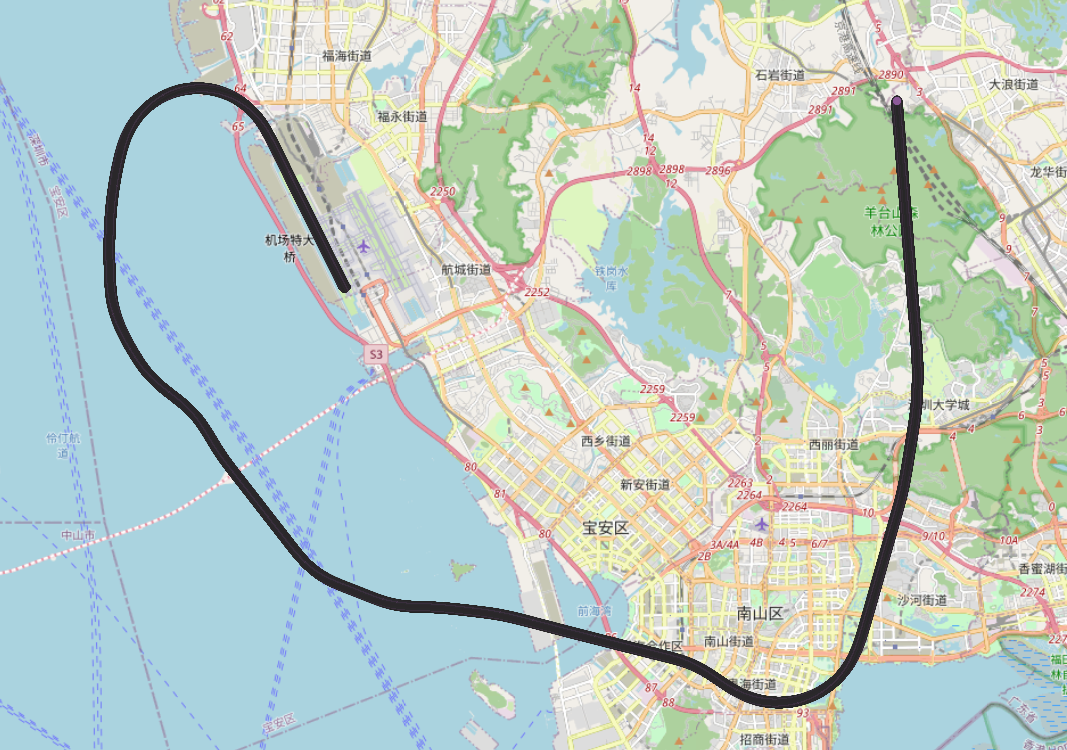
\includegraphics[width=.9\textwidth]{pictures/trace.png}
        \caption{GIS绘制路径}
        \label{GIStrace}
    \end{center}
\end{figure}
\par
以上是对于最重要的飞行指令的验证过程,而对于设置灯光、天气等指令的验证可以通过手动操作变化,检查捕获到的数据帧中的变化进行验证。
文档中给出的CAE仿真机指令共有近70条,由于文档老旧,其中有些指令已经停用,同时也有文档中并不存在的指令。好在目前阶段通过结合文档和飞行员经验,已有21条仿真机控制指令和5条视景系统反馈指令通过验证,其中囊括了飞机地理位置、机身灯光、雨雪天气、能见度等指令,也包含了如碰撞提示等反馈指令。
这些指令能保障视景系统中如飞行、天气变化、碰撞检测等基本功能的实现。
表\ref{caecommand}列举了已成功验证的部分仿真机指令代号及功能。


% \section{视景系统整体概述}
% 视景系统是FFS中负责连续生成模拟座舱前方飞行画面的系统。飞行员在模拟座舱中的操作将作为仿真机的输入,经过模拟计算后输出如位置、姿态、灯光等一系列指令,图像生成器根据指令要求执行逻辑后便可渲染连贯的飞行画面,提供模拟飞行的视觉效果。
% 同时图像生成器也要以指令的形式反馈给仿真机如碰撞等信息。仿真机可以据此通知如声音、运动系统做出相应反馈。
% \par
% 由上述可知仿真机相当于FFS的服务端,视景系统类似客户端,但此案例的服务端与客户端在网络体系结构中处于不同层级,需要请一个翻译才能正常进行数据交换,本系统中将该翻译角色称为虚拟仿真机。
% 视景系统整体架构如图\ref{framework}所示。仿真机作为一个底层网络设备,其只能接收或发送仅用以太网协议封装的数据包,且使用该公司自定义的数据交换协议;虚拟仿真机作为翻译需要对双方的消息解封、转换再封装,最后发送。同时在没有仿真机的开发环境下也可以读取模拟数据实现流程;
% 虚拟仿真机与客户端之间使用ProtoBuffer作为数据交换协议,TCP通信任务由Tbuspp插件承担。图像生成器需要根据收到的指令先完成数据同步工作,再执行逻辑,计算反馈信息。图中虚线框中的部分包含了数据由仿真机到图像生成器中被使用,生成的反馈信息再最终回到仿真机的全过程,此部分便是视景系统中的数据交换子系统。
% \par
% 图像生成器中还含有许多重要的功能组成部分。首先引擎核心为其提供了渲染、物理、脚本、数学计算等运行核心组件,许多逻辑依赖其中的方法实现,逻辑执行结束后也需要渲染介入。
% 机场资产则是场景的数据库,地形、建筑、纹理等资源皆存于其中,需要根据飞机所处位置去查找并加载这些资源,这对于数据的组织形式,查找策略都有较高的要求。
% 投影同步插件负责在FFS上运行时控制多台投影仪投影相同的一帧以减少画面撕裂,另外由于模拟座舱前方是一个球幕,需要校准球幕投影时发生的畸变。

\section{基础数据交换需求分析}
确定了仿真机与原视景系统间的指令沟通方式后,便可以开展数据交换子系统的设计与实现工作。系统设计的第一步是需求分析,其主要目的是明晰非形式化
的需求,最终产生完整的需求规格说明。本节首先分析了系统中的涉众,阐述了涉众对系统的期望。
随后从系统的角度解释软件,定义了系统的功能性需求和非功能性需求。
最后在理解需求的基础上,设计了多个系统用例,并使用4+1视图确定了系统的整体结构。
\begin{table}[h!]
    \begin{center}
        \caption{仿真机部分指令列表}
        \label{caecommand}
        \renewcommand\arraystretch{1.5}
        \begin{tabularx}{0.8\textwidth}{ 
            | >{\centering\arraybackslash\hsize=.15\hsize\linewidth=\hsize}X 
            | >{\raggedright\arraybackslash\hsize=.85\hsize\linewidth=\hsize}X 
            | }
            \hline
            \textbf{代号} & \textbf{指令用途}\\
            \hline
            21H &  负责控制飞机的位置与飞行姿态,是仿真机每帧都要更新的最基本指令,其通过经纬度海拔确定位置,通过该位置东北天坐标系下的欧拉角确定姿态。\\
            \hline
            42H &  负责控制机身主要位置灯光开关和照明角度,指令中包含灯光的状态和相对机身水平竖直方向的两个角度。\\
            \hline
            43H &  负责控制机场灯光,指令中包括跑道滑行灯、PAPI灯、四组不同距离的环境灯等灯光的状态。\\
            \hline
            44H &  负责部分天气效果的控制,指令中包含下雨、下雪及其程度的描述,云层的效果等信息。\\
            \hline
            45H &  负责能见度的控制,指令中包含雾的浓度,可视角度等信息,在盲降训练时会被使用。\\
            \hline
            47H &  负责所处时间段的控制,指令中包含白昼、黑夜、黎明、黄昏四种时间段信息,且根据不同的日期会有不同的太阳高度和月相信息。反映到视景系统中会产生不同的天光。\\
            \hline
            86H &  负责一些通用信息的反馈,包括视景中使用的地球坐标系类型,当前加载的机场编号,是否发生严重碰撞等等。\\
            \hline
            82H &  负责反馈飞机上某点的离地高度,一般是用于降落时起落架相关信息的计算。\\
            \hline
        \end{tabularx}
    \end{center}
\end{table}
\subsection{涉众分析}
本系统作为视景系统中负责数据交换的子系统,参与者主要有二,一是每帧产生各种指令数据的仿真机,二是负责根据收到的指令执行逻辑并完成渲染的图像生成器。
仿真机和图像生成器都希望有一座桥梁协助进行双向交流,以实现最终飞行画面的渲染。
详细的涉众分析如表\ref{stakeholder}所示。
\begin{table}[h!]
    \begin{center}
        \caption{涉众分析列表}
        \label{stakeholder}
        \renewcommand\arraystretch{1.5}
        \begin{tabularx}{\textwidth}{ 
            | >{\centering\arraybackslash\hsize=.25\hsize\linewidth=\hsize}X 
            | >{\raggedright\arraybackslash\hsize=.75\hsize\linewidth=\hsize}X 
            | }
            \hline
            \textbf{涉众名称} & \textbf{涉众期望}\\
            \hline
            仿真机 &      仿真机作为驱动图像生成器工作的数据源头,希望自己每一帧产生的指令数据能被图像生成器及时接收并正确解读。
                          同时希望收到图像生成器的反馈信息以联动其他系统作出反应。\\
            \hline
            图像生成器 &  图像生成器作为执行逻辑和渲染画面的角色,希望从仿真机处取得指令数据,使用其中的数据完成逻辑计算。
                         同时需要将产生的反馈数据发送给到仿真机。另外本视景系统中的图像生成器希望有搭载于不同仿真机上的能力。\\
            \hline
        \end{tabularx}
    \end{center}
\end{table}
\subsection{功能性需求}
图像生成器依据仿真机指令进行飞行画面渲染并反馈飞行数据,要求仿真机与图像生成器之间进行双向数据交换。上一节中对仿真机的分析里提到,仿真机网络协议栈简单,其输出与输入均为只用以太网协议封装的数据帧,这种数据帧不能交由一般的网络协议栈处理,
需要自己实现针对该数据帧的解封和封装过程,转换为自定义指令后的数据则可以通过TCP协议栈发送给图像生成器。我们将中间的桥梁称为虚拟仿真机。另外图像生成器需要在没有仿真机的开发条件下使用模拟数据帧驱动逻辑运转。

% 在信息的传输过程中避免不了存在网络波动;且虚拟仿真机与图像生成器间用无法广播的TCP协议通信,对于单一图像生成器而言数据到达频率可能不稳定,对于多个图像生成器而言同一数据到达时刻也不相同。
% 因此需要进行数据同步抵消差异。另外从单一图像生成器角度,逻辑帧的开始时间受渲染帧约束,不能保证绝对稳定,如果按照仿真机的原始数据飞行可能会产生不自然的闯动,需要一定的数据平滑策略减少影响。
在本视景系统中具体得到数据流动可用下面这一完整流程描述:
\begin{itemize}
    \item [(1)]
    仿真机根据飞行员的输入计算飞行状态,产生一条条指令数据,将这些指令数据仅通过以太网协议封装后以数据链路层数据帧的形式输出。
    \item [(2)]
    虚拟仿真机接收数据链路层数据帧,去除以太网协议的头尾内容,完成解封。识别指令代号后,直接使用对应结构体反序列化指令内容。
    \item [(3)]
    将指令中特殊数字表示方式下的数据通过算法转换为便于图像生成器使用的数字形式。如将经度0000007f ffffffff转换为179.99后,结合纬度和海拔信息转换为笛卡尔坐标系位置,再赋值给自定义指令中的对应字段,生成我们自定义的指令集。
    \item [(4)]
    将该自定义指令通过数据交换协议进行序列化,并通过TCP协议发送给图像生成器,此过程中的网络协议封装则全权交由操作系统的内核网络协议栈完成。
    \item [(5)]
    图像生成器接收到数据后,同样由内核网络协议栈解封,再使用同样的交换协议反序列化得到指令结构化数据,供给逻辑线程使用。
    \item [(6)]
    图像生成器的反馈信息则通过完全相反的过程,最终逆向发送到仿真机。
\end{itemize}


\par
% 另外数据交换子系统作为视景系统的一部分,流经它的数据最终要服务于视景系统中的部分逻辑,且反馈数据也来自于逻辑执行。
% 但项目初始阶段视景系统中并不存在任何运行逻辑,因此我们将飞行模拟最基础的飞机飞行一系列逻辑作为数据交换子系统的部分功能。它将使用接收到的指令完成飞行,并将检测到的地形信息作为反馈。
% 最终飞行画面是否正确、流畅也是判断数据交换子系统是否正常运作的重要依据。
整个指令数据传输的过程中需要保证虚拟仿真机与图像生成器依照仿真机的工作频率运行,即数据到达便要处理并发送,这个过程中有一些缓存机制需要禁用。
数据交换子系统的功能性需求列表如表\ref{funcreq}所示。
\begin{table}[h!]
    \begin{center}
        \caption{系统功能性需求列表}
        \label{funcreq}
        \renewcommand\arraystretch{1.5}
        \begin{tabularx}{\textwidth}{ 
            | >{\centering\arraybackslash\hsize=.1\hsize\linewidth=\hsize}X 
            | >{\centering\arraybackslash\hsize=.3\hsize\linewidth=\hsize}X 
            | >{\raggedright\arraybackslash\hsize=.6\hsize\linewidth=\hsize}X 
            | }
            \hline
            \textbf{ID} & \textbf{需求名称} & \textbf{需求描述}\\
            \hline
            R1 & 仿真机与虚拟仿真机交互 & 由于仿真机数据帧的特性,虚拟仿真机需要绕过所在操作系统的网络协议栈,直接读取或生成流经网卡的原始数据帧,需要亲自实现解封和封装数据帧的过程。
                                        此过程中需要按照仿真机的发送频率读取网卡数据,确保指令数据的实时性。\\
            \hline
            R2 & 指令数据转换 & 仿真机使用的指令需要与图像生成器使用的指令进行映射,同时需要进行数字表示方法的转换,方便双方对于指令数据的使用。\\
            \hline 
            R3 & 图像生成器与虚拟仿真机交互 & 图像生成器可以与虚拟仿真机以自定义指令的格式进行交互,图像生成器需要正确识别指令类型。\\
            % \hline 
            % R4 & 数据同步与平滑 & 图像生成器不可以立即使用到达的数据指令,存储几帧内容与其他机器进行同步处理。图像生成器可以对存储的内容进行平滑,减少逻辑帧的不稳定带来的抖动。\\
            \hline
        \end{tabularx}
    \end{center}
\end{table}


\subsection{非功能性需求}
帧率是动态画面视觉体验的重要因素,对于电视与电影这类视频行业来讲24Hz以上的帧率便能达到良好的观看体验\cite{frame}。但对于需要飞行员实施操控的飞行模拟而言,60Hz以上的帧率才不会让飞行员产生操作延迟的感觉,因此本视景系统初期要求在训练基地的FFS设备上能达到60Hz的帧率,且运行时不出现可观察到的抖动现象。
目前国内的进口模拟机来自CAE等外国公司,虽然各厂商的仿真机都是数据链路层设备,但他们的指令有不同的数据组织结构和数字表示方法。表\ref{simsattr}展示了CAE公司与Flight Safety公司仿真机关于飞机地理位置的指令结构对比,它们在组织结构上存在明显差异,且其中的数字解释方法不尽相同。数据交换子系统需要屏蔽这些差异,方便日后的二次开发以适配不同仿真机。系统的非功能性需求列表如表\ref{unfuncreq}所示。
\begin{table}[htbp]
    \begin{center}
        \caption{不同仿真机字段比较}
        \label{simsattr}
        \renewcommand\arraystretch{1.2}
        \begin{tabularx}{\textwidth}{ 
            | >{\centering\arraybackslash\hsize=\hsize\linewidth=\hsize}X 
            | >{\centering\arraybackslash\hsize=\hsize\linewidth=\hsize}X 
            | >{\centering\arraybackslash\hsize=\hsize\linewidth=\hsize}X 
            | >{\centering\arraybackslash\hsize=\hsize\linewidth=\hsize}X 
            | }
            \hline
            \textbf{CAE字段} & \textbf{长度} & \textbf{FS字段} & \textbf{长度}\\
            \hline
            OpCode & 16bit & Packet ID & 16bit\\
            \hline
            CS number & 32bit & Entity ID & 16bit\\
            \hline
            Latitude MSW & 32bit & Roll & 32bit\\
            \hline
            Latitude LSW & 32bit & Pitch & 32bit\\
            \hline
            Longitude MSW & 32bit & Yaw & 32bit\\
            \hline
            Longitude LSW & 32bit & Latitude & 64bit\\
            \hline
            Altitude& 32bit & Longitude & 64bit\\
            \hline
            Roll & 32bit & Altitude & 32bit\\
            \hline
            Pitch& 32bit &  etc. & \\
            \hline
            Yaw & 32bit &  & \\
            \hline
            etc. & &  & \\
            \hline
        \end{tabularx}
    \end{center}
\end{table}
\begin{table}[h!]
    \begin{center}
        \caption{系统非功能性需求列表}
        \label{unfuncreq}
        \renewcommand\arraystretch{1.5}
        \begin{tabularx}{\textwidth}{ 
            | >{\centering\arraybackslash\hsize=.1\hsize\linewidth=\hsize}X 
            | >{\centering\arraybackslash\hsize=.3\hsize\linewidth=\hsize}X 
            | >{\raggedright\arraybackslash\hsize=.6\hsize\linewidth=\hsize}X 
            | }
            \hline
            \textbf{ID} & \textbf{需求名称} & \textbf{需求描述}\\
            \hline
            R1 & 运行帧率 & 飞行画面在60Hz以上才不会产生明显操作延迟感,因此要求初期在真实FFS设备上能够达到最低60Hz的渲染帧率,也意味着数据交换子系统能够以这个频率处理数据。且日后经游戏引擎角度的不断优化能够达到100Hz以上。\\
            \hline
            R2 & 可靠性 & 一次飞行训练课持续50分钟,要求视景系统在连续运行30分钟期间不出现明显的画面撕裂、抖动和帧率下降趋势。\\
            \hline
            R3 & 可扩展性 & 由于国内现存各厂商的仿真机均使用自定义数据组织结构和数字表示方法,数据交换子系统应体现仿真机侧无关性,将不同厂商的指令映射为我们自定义的指令集,方便经过二次开发后在各类仿真机上搭载。\\
            \hline
        \end{tabularx}
    \end{center}
\end{table}

\subsection{用例设计}
理解了非形式化的需求后便可以根据需求设计具体用例。图\ref{sysedge}展示了数据交换子系统的边界,确定了其在视景系统中的所处位置。
首先我们并不关心仿真机中的指令数据如何产生,只需要接收或发送仅用以太网协议封装过的数据帧。数据经过虚拟仿真机一系列处理后通过TCP协议发送给图像生成器,图像生成器解析出指令数据后给到逻辑部分使用,从此走出子系统边界。当然逻辑执行完后还需要将结果交给资产管理和引擎核心部分实现场景加载和渲染。
系统的功能集中在整个虚拟仿真机和图像生成器中的通信部分。

\begin{figure}[h]
    \begin{center}
        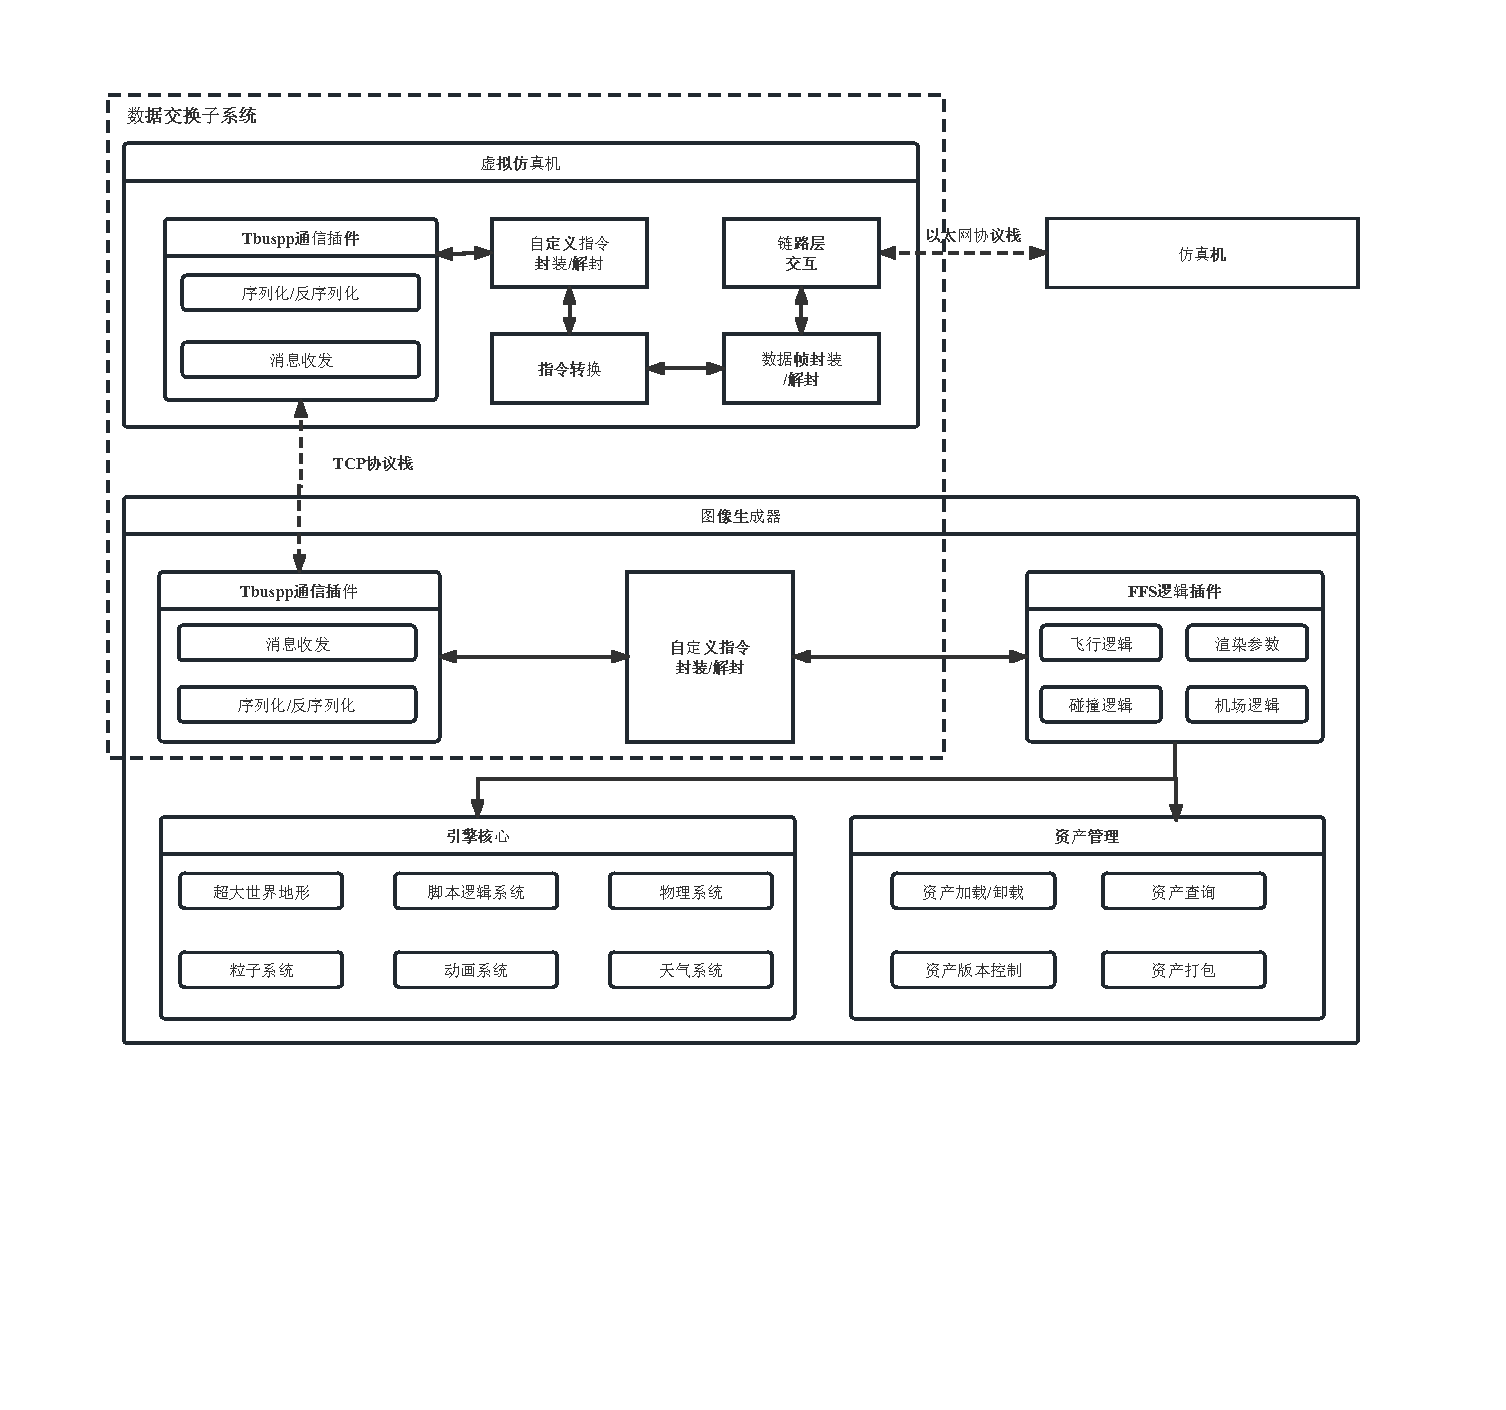
\includegraphics[width=\textwidth]{pictures/sysedge.pdf}
        \caption{数据交换子系统边界}
        \label{sysedge}
    \end{center}
\end{figure}
\par
经过需求分析后最终确定将数据交换子系统划分为七个用例,系统用例图如图\ref{usecase}所示。其中的角色分为仿真机和图像生成器。
仿真机与虚拟仿真机建立数据链路层连接,并使用各自的指令交互。仿真机中的指令数据经过解封、转换、封装等一系列动作后变为一个自定义指令,序列化后通过Tbuspp发送给图像生成器;
图像生成器接收数据后,根据反序列化后得到的指令内容执行逻辑,逻辑执行的结果最终用于加载对应资源和渲染画面等过程。
飞行中产生的反馈信息则由图像生成器逆向发送最终以仿真机指令的形式给到仿真机。
\par
具体而言,仿真机的用例包括建立链路层连接、发送数据帧、收取数据帧、以及指令格式转换。
图像生成器的用例包括收发Tbuspp消息、自定义指令的封装与解封、指令格式转换和使用模拟数据。



\begin{figure}[h!]
    \begin{center}
        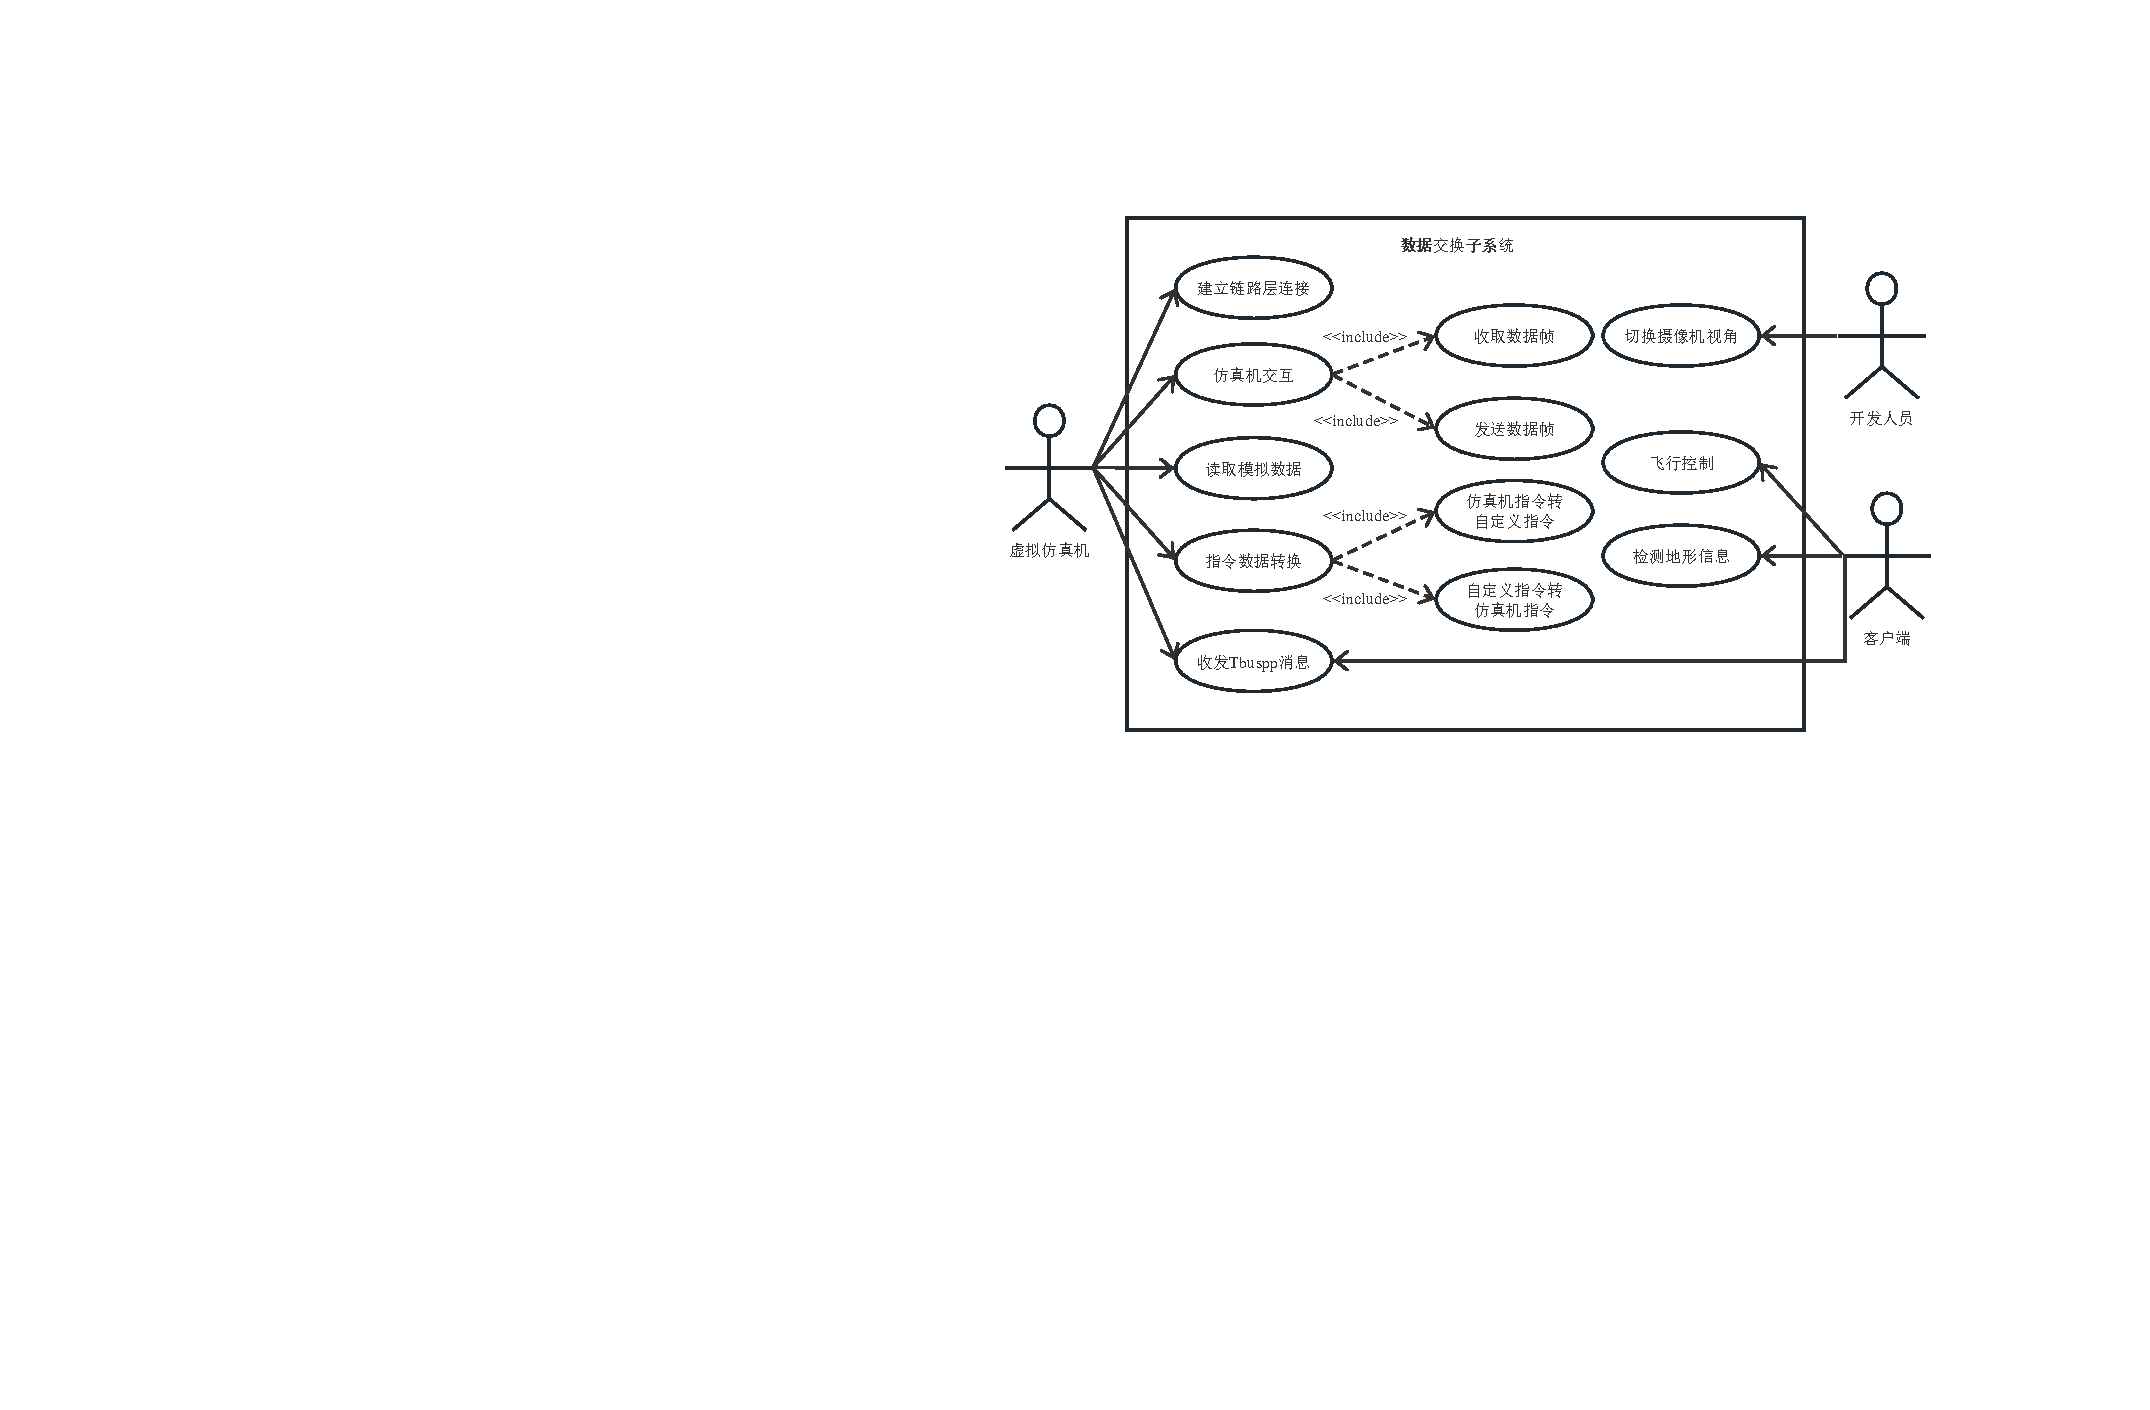
\includegraphics[width=0.8\textwidth]{pictures/usecase.pdf}
        \caption{数据交换子系统用例图}
        \label{usecase}
    \end{center}
\end{figure}

\par
下面将对用例图中提到的系统用例通过用例描述表的形式进行详细解释。
\par
建立链路层连接,是仿真机与虚拟仿真机建立沟通路径的方式。由于仿真机简单的网路协议栈,其产生的数据帧不含有IP头、TCP头等信息,
与仿真机相关的数据不能直接由虚拟仿真机运行环境中的网络协议栈处理,必须由虚拟仿真机亲自侦听网卡上的原始数据帧,并实现解封或封装。
另需额外注意侦听数据时要使用及时转发模式,否则网卡的缓存机制会降低侦听的频率,产生较大的延迟,最终影响到图像的生成。用例的具体情况如表\ref{usecase1}所示。
\clearpage
\begin{table}[htbp]
    \begin{center}
        \caption{建立链路层连接用例描述表}
        \label{usecase1}
        \renewcommand\arraystretch{1.5}
        \begin{tabularx}{0.8\textwidth}{ 
            | >{\centering\arraybackslash\hsize=.5\hsize\linewidth=\hsize}X 
            | >{\raggedright\arraybackslash\hsize=1.5\hsize\linewidth=\hsize}X 
            | }
            \hline
            \textbf{ID} & \textbf{UC1}\\
            \hline
            参与者 & 仿真机\\
            \hline
            触发条件 & 视景系统开始运行。\\
            \hline
            前置条件 & 虚拟仿真机处于接收仿真机消息模式。\\
            \hline
            后置条件 & 能够与虚拟仿真机进行数据交流。\\
            \hline
            优先级 & 高\\
            \hline
            正常流程 &  1.查找运行环境下的网络适配器列表。\par 2.选择其中一个网络适配器。\par 3.获取混杂模式数据包捕获句柄。\par 4. 开启及时转发模式。\\
            \hline
            扩展流程 & 网络适配器不能正常运作,打印错误提示。\\
            \hline
        \end{tabularx}
    \end{center}
\end{table}
\par
发送数据帧,是仿真机将数据帧发送到虚拟仿真机的过程。虚拟仿真机侦听到数据到来后不依靠网络协议栈自动解封,而是自己实现解封过程。收取具体情况如表\ref{usecase2}所示。
\begin{table}[htbp]
    \begin{center}
        \caption{发送数据帧用例描述表}
        \label{usecase2}
        \renewcommand\arraystretch{1.5}
        \begin{tabularx}{0.8\textwidth}{ 
            | >{\centering\arraybackslash\hsize=.5\hsize\linewidth=\hsize}X 
            | >{\raggedright\arraybackslash\hsize=1.5\hsize\linewidth=\hsize}X 
            | }
            \hline
            \textbf{ID} & \textbf{UC2}\\
            \hline
            参与者 & 仿真机\\
            \hline
            触发条件 & 仿真机向虚拟仿真机发送数据帧。\\
            \hline
            前置条件 & 虚拟仿真机侦听了正确的网卡。\\
            \hline
            后置条件 & 数据帧被分为一个个指令数据段。\\
            \hline
            优先级 & 高\\
            \hline
            正常流程 & 1.仿真机发送数据帧。 \par 2.虚拟仿真机去除数据帧头部信息。\par 3.读取指令长度信息并按该长度截取。\par 4.将数据段加入仿真机指令集合。\par 5.回到流程3循环至全部数据读取结束。\\
            \hline
            扩展流程 & 无\\
            \hline
        \end{tabularx}
    \end{center}
\end{table}
\par
收取数据帧,是仿真机收取反馈信息的过程,此过程虚拟仿真机同样不依靠网络协议栈自动封装,而是自己实现封装过程。具体情况如表\ref{usecase3}所示。
\begin{table}[htbp]
    \begin{center}
        \caption{发送数据帧用例描述表}
        \label{usecase3}
        \renewcommand\arraystretch{1.5}
        \begin{tabularx}{0.8\textwidth}{ 
            | >{\centering\arraybackslash\hsize=.5\hsize\linewidth=\hsize}X 
            | >{\raggedright\arraybackslash\hsize=1.5\hsize\linewidth=\hsize}X 
            | }
            \hline
            \textbf{ID} & \textbf{UC3}\\
            \hline
            参与者 & 仿真机\\
            \hline
            触发条件 & 仿真机反馈指令到达。\\
            \hline
            前置条件 & 虚拟仿真机侦听了正确的网卡。\\
            \hline
            后置条件 & 仿真机收到视景系统反馈并通知其它系统协同。\\
            \hline
            优先级 & 高\\
            \hline
            正常流程 & 1.反馈指令数据段到达。\par 2.将多条指令按规则粘合在一个数据包中。\par 3.为数据包添加以太网头尾信息。\par 4.将数据帧发送给仿真机。\\
            \hline
            扩展流程 & 无。\\
            \hline
        \end{tabularx}
    \end{center}
\end{table}
\par
国内的FFS全部位于航空公司的训练基地内,其价格昂贵且庞大,是及其珍贵的训练资源,无法搬运至开发环境中。在日常开发中,虚拟模拟机需要读取文件中的模拟数据来驱动视景系统运作。具体情况如表\ref{usecase4}所示。
\begin{table}[htbp]
    \begin{center}
        \caption{使用模拟数据用例描述表}
        \label{usecase4}
        \renewcommand\arraystretch{1.5}
        \begin{tabularx}{0.8\textwidth}{ 
            | >{\centering\arraybackslash\hsize=.5\hsize\linewidth=\hsize}X 
            | >{\raggedright\arraybackslash\hsize=1.5\hsize\linewidth=\hsize}X 
            | }
            \hline
            \textbf{ID} & \textbf{UC4}\\
            \hline
            参与者 & 图像生成器\\
            \hline
            触发条件 & 使用模拟数据驱动图像生成器运作。\\
            \hline
            前置条件 & 虚拟仿真机处于读取模拟数据模式。\\
            \hline
            后置条件 & 文本信息被转化为仿真机数据帧信息。\\
            \hline
            优先级 & 高\\
            \hline
            正常流程 & 1.指定文件路径。\par 2.虚拟仿真机按行读取文本。\par 3.将字符两两一组转换为一个字节。\par 4.按用例2中的流程进行。\\
            \hline
            扩展流程 & 文件不存在或格式有错误则产生警告。\\
            \hline
        \end{tabularx}
    \end{center}
\end{table}
\par
指令格式转换用例,描述了是仿真机指令与自定义指令相互转换的过程,转换后的指令格式更适合另一方使用。由于其流程类似,将两方的转换过程合并为同一个用例。具体情况如表\ref{usecase5}所示。
\begin{table}[htbp]
    \begin{center}
        \caption{指令格式转换用例描述表}
        \label{usecase5}
        \renewcommand\arraystretch{1.5}
        \begin{tabularx}{0.8\textwidth}{ 
            | >{\centering\arraybackslash\hsize=.5\hsize\linewidth=\hsize}X 
            | >{\raggedright\arraybackslash\hsize=1.5\hsize\linewidth=\hsize}X 
            | }
            \hline
            \textbf{ID} & \textbf{UC5}\\
            \hline
            参与者 & 仿真机\&图像生成器\\
            \hline
            触发条件 & 存在待转换的指令。\\
            \hline
            前置条件 & 注册了该指令的转换器。\\
            \hline
            后置条件 & 构建出自定义指令/仿真机指令。\\
            \hline
            优先级 & 高\\
            \hline
            正常流程 &  1.获取指令结构中的指令代号。\par 2.根据指令代号查找对应的转换器。\par 3.使用转换器完成转换。\\
            \hline
            扩展流程 & 对于暂时使用不到的不存在转换器的指令直接丢弃。\\
            \hline
        \end{tabularx}
    \end{center}
\end{table}
\par
ProtoBuffer作为二进制数据交换协议,面对多种指令同样需要一个代号来决定使用何种结构
反序列化指令字段。因此需要为自定义指令额外封装指令代号等信息,构成一个通用结构,整个过程需要两次序列化。
作为接收方则同样需要两次反序列化。具体情况如表\ref{usecase6}所示。
\begin{table}[htbp]
    \begin{center}
        \caption{自定义指令封装用例描述表}
        \label{usecase6}
        \renewcommand\arraystretch{1.5}
        \begin{tabularx}{0.8\textwidth}{ 
            | >{\centering\arraybackslash\hsize=.5\hsize\linewidth=\hsize}X 
            | >{\raggedright\arraybackslash\hsize=1.5\hsize\linewidth=\hsize}X 
            | }
            \hline
            \textbf{ID} & \textbf{UC6}\\
            \hline
            参与者 & 图像生成器\\
            \hline
            触发条件 & 图像生成器需要发送或接收自定义指令。\\
            \hline
            后置条件 & 自定义指令被封装并序列化。\\
            \hline
            优先级 & 高\\
            \hline
            正常流程 & 
                    %   封装过程:\par 1.为指令添加代号等信息,得到通用结构。\par 2.将整个结构序列化。\par 
                      1.将自定义指令序列化。\par 2.为序列化后的包添加代号等信息,构成通用结构。\par 3.将通用结构再次序列化。\\
            % \hline
            % 扩展流程 & 无\\
            \hline
        \end{tabularx}
    \end{center}
\end{table}
\par
图像生成器与虚拟仿真机利用Tbuspp插件进行沟通,双方都需要对Tbuspp消息进行收发。具体情况如表\ref{usecase7}所示。
\begin{table}[htbp]
    \begin{center}
        \caption{收发Tbuspp消息用例描述表}
        \label{usecase7}
        \renewcommand\arraystretch{1.5}
        \begin{tabularx}{0.8\textwidth}{ 
            | >{\centering\arraybackslash\hsize=.5\hsize\linewidth=\hsize}X 
            | >{\raggedright\arraybackslash\hsize=1.5\hsize\linewidth=\hsize}X 
            | }
            \hline
            \textbf{ID} & \textbf{UC7}\\
            \hline
            参与者 & 图像生成器\\
            \hline
            触发条件 & 有通用结构待发送。\\
            \hline
            前置条件 & Tbuspp连接成功建立。\\
            \hline
            后置条件 & 无\\
            \hline
            优先级 & 高\\
            \hline
            正常流程 &  数据发送过程:\par 1.用ProtoBuffer协议序列化通用结构。\par 2.将消息写入Tbuspp发送队列。\par 
                       数据接收过程:\par 1.从Tbuspp接收队列读取消息。\par   2.使用通用结构反序列化该消息。\\
            \hline
            扩展流程 & Tbuspp连接失败产生警告。\\
            \hline
        \end{tabularx}
    \end{center}
\end{table}

\section{基础数据交换概要设计}
数据交换子系统的架构设计如图\ref{subframe}所示,整个系统分为三个部分,数据交换的功能集中于虚拟仿真机与图像生成器中。仿真机与虚拟仿真机间通过数据链路层协议进行交互,虚拟仿真机与图像生成器通过TCP协议交互。
仿真机的作用是对飞行员的操作输入进行仿真计算,得出飞机状态,这部分由FFS厂商设计开发。虚拟仿真机则将仿真机指令翻译为图像生成器方便使用的自定义指令,使用自定义指令同时屏蔽了不同仿真机的差异。
图像生成器需要按照收到的指令数据进行逻辑演算并渲染飞行画面,并提供飞行中的反馈信息。
\par
功能主要分为三个模块,分别是仿真机侧数据交换模块,指令转换模块和图像生成器侧数据交换模块。
仿真机侧数据交换模块负责处理与仿真机进行交流的全部任务。其中使用到WinPcap作为直接访问网卡的工具,数据帧的收取和发送都通过WinPcap实现。
为处理仿真机的特殊数据帧,需要自己实现数据帧的解封和封装逻辑。指令转换模块是一个承上启下的模块,其负责仿真机指令与自定义指令间的转换。
其中涉及到数字表示方式的变化和如经纬海拔与笛卡尔坐标系转换的算法。此模块不仅提供翻译功能,作为视景系统的一部分,其屏蔽了仿真机侧指令的差异。
图像生成器侧数据交换模块负责处理与图像生成器进行交流的全部任务,此处的通信则使用常规的TCP协议,不再需要亲自实现网络协议栈。
此处的数据交换协议使用二进制协议ProtoBuffer,其拥有非常高的序列化反序列化速度,以及相当小的序列化体积,适合交换频率高的场景。
图像生成器中也有一个类似的模块负责与虚拟仿真机交流。
% 仿真机的运行频率为60Hz,虚拟仿真机使用收到即处理的策略,图像生成器的渲染帧率同样限制为60Hz,
\par 
数据交换子系统完全使用C++语言开发,图像生成器中核心功能如通用坐标系转换、射线探测等由C++语言开发。模拟飞行视景系统的专属逻辑如飞行控制则使用Lua脚本嵌入,方便修改。


\begin{figure}[htbp]
    \begin{center}
        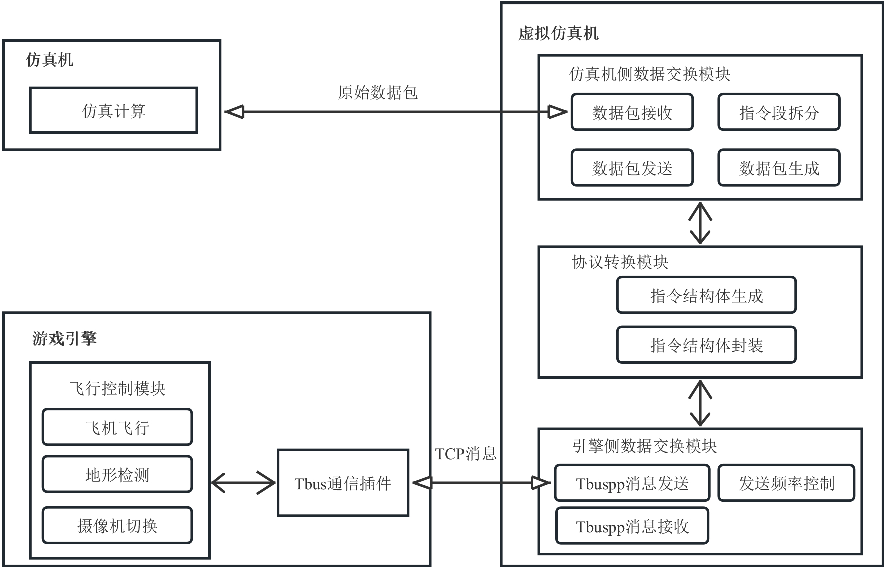
\includegraphics[width=\textwidth]{pictures/framework.pdf}
        \caption{数据交换子系统架构图}
        \label{subframe}
    \end{center}
\end{figure}
\subsection{系统逻辑视图}
逻辑视图以用户为中心,以类图的形式展示了系统的架构和功能模块。系统通过逻辑层次划分,把各个功能抽象成类,实现功能的封装。
如图\ref{logic}为数据交换子系统的逻辑视图。SimNodeContext代表仿真机与虚拟仿真机间沟通的环境,其中依赖MacLinkLayer类,负责建立维持底层网络的连接,兼顾数据帧收发过程的实现;
MacReceive和MacSend分别表示虚拟仿真机接收和发送数据帧的线程,MacReceive线程会持续运行,当MacLinkLayer收到数据帧后,该线程会立即对其处理,再交给Convertor模块转换。MacSend则会在收到Convertor的数据后进行封装,再交给MacLinkLayer执行发送。
\par
Convertor表示指令转换模块。仿真机和图像生成器都无法直接使用对方生成的指令信息,因此需要该模块对双方的指令按照规则转换。
IProtoclConversion是一个模板类,Convertor通过实例化该模板,表示一对指令间的转换。在初始化时需要完成对于所有Convertor的注册。Utils类中则是一些特殊的数字表示方式转换算法。
\par
ImageGeneratorContext表示虚拟仿真机与图像生成器间沟通的模块,该模块的通信使用Tbuspp插件实现TCP通信,FFSDevice是对图像生成器的抽象,在搭配不同仿真机的情况下会使用不同的Convertor集合进行指令转换。
IGReceive和IGSend分别表示图像生成器接收和发送消息的线程。当收到来自Tbuspp的消息时,会将其交给Handler首先解读出指令代号,再使用对应结构反序列化。当有序列化完毕的消息发送时则由IGSend写入Tbuspp的发送队列。
\begin{figure}[h]
    \begin{center}
        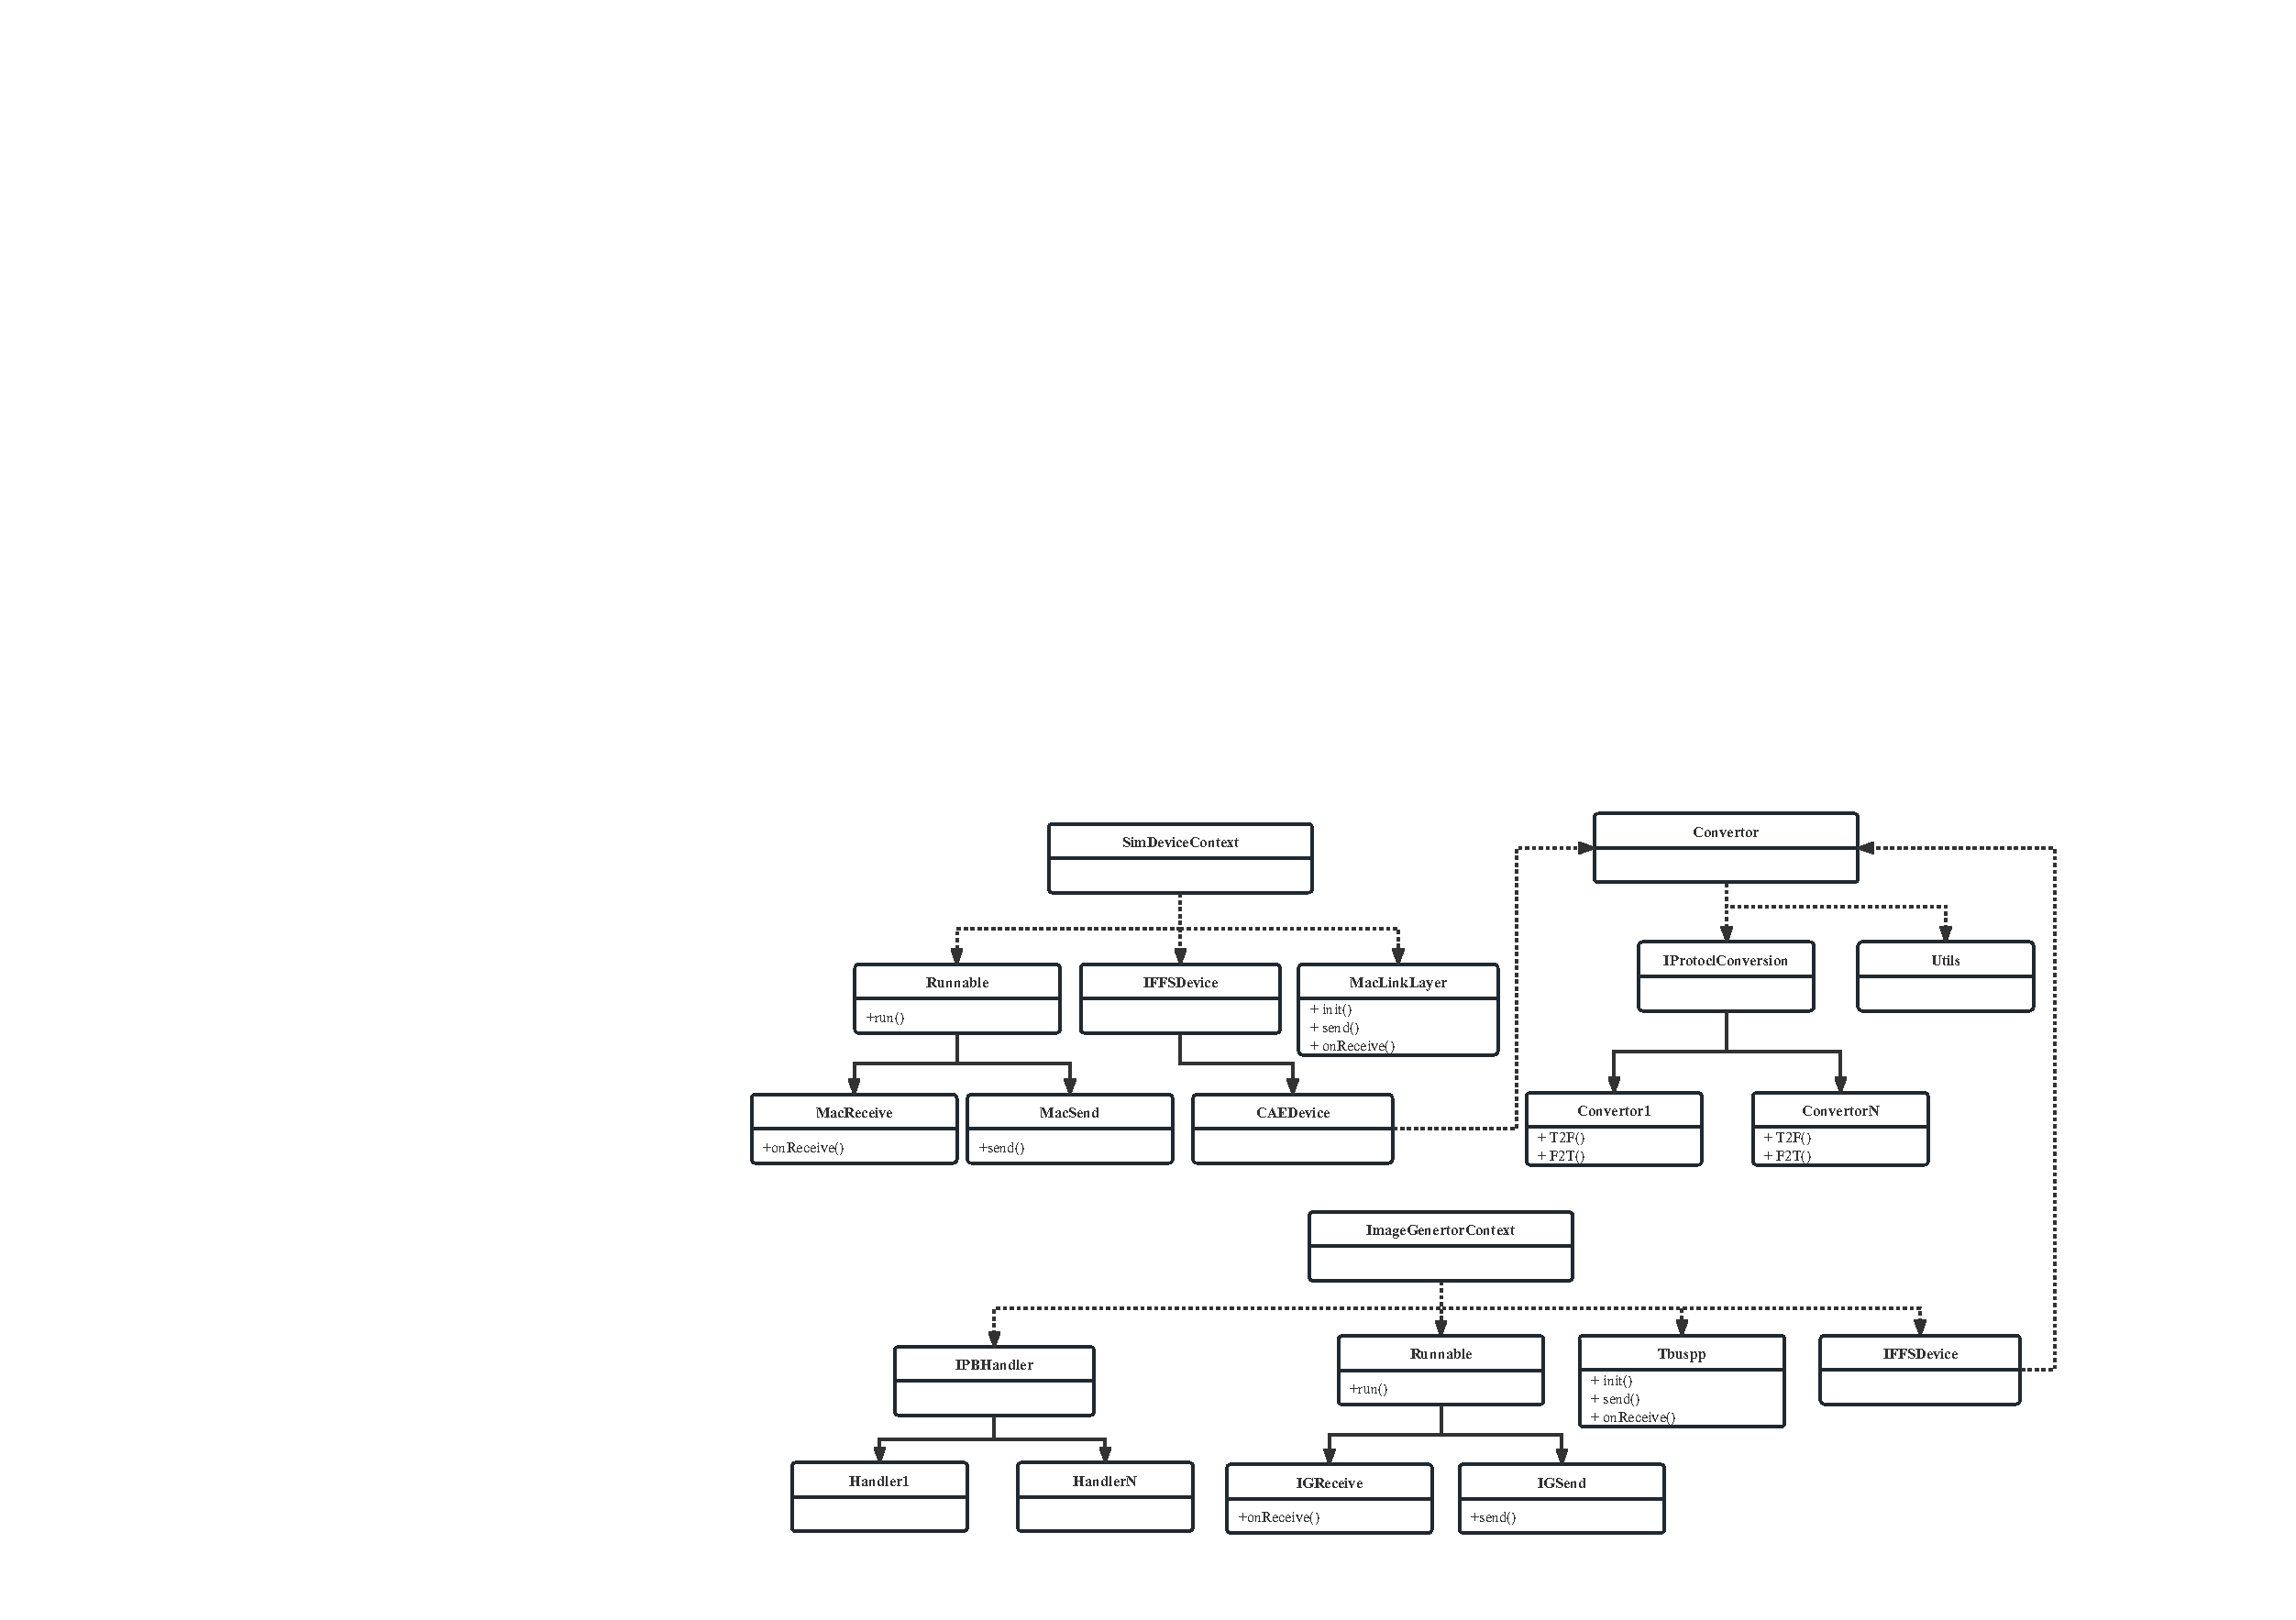
\includegraphics[width=\textwidth]{pictures/logic.pdf}
        \caption{逻辑视图}
        \label{logic}
    \end{center}
\end{figure}
\subsection{系统开发视图}
开发视图注重描述软件开发过程中实际模块的组织,反映了系统工程的具体实施过程。
本系统的开发视图如图\ref{dev}所示,虚拟仿真机接收来自仿真机这一服务端的信息,其中处理过程分为三层。
第一层负责与仿真机交流,使用交流环境到线程实例到具体设备再到链路层连接的结构进行数据帧收发的处理。
中间层负责对双方指令的转换,其中使用到策略模式实现繁多指令间的转化。
第三层负责图像生成器的交流,同样使用环境到线程实例到设备再到具体连接的结构进行开发,图像生成器中另外含有使用数据的逻辑部分。
\begin{figure}[h]
    \begin{center}
        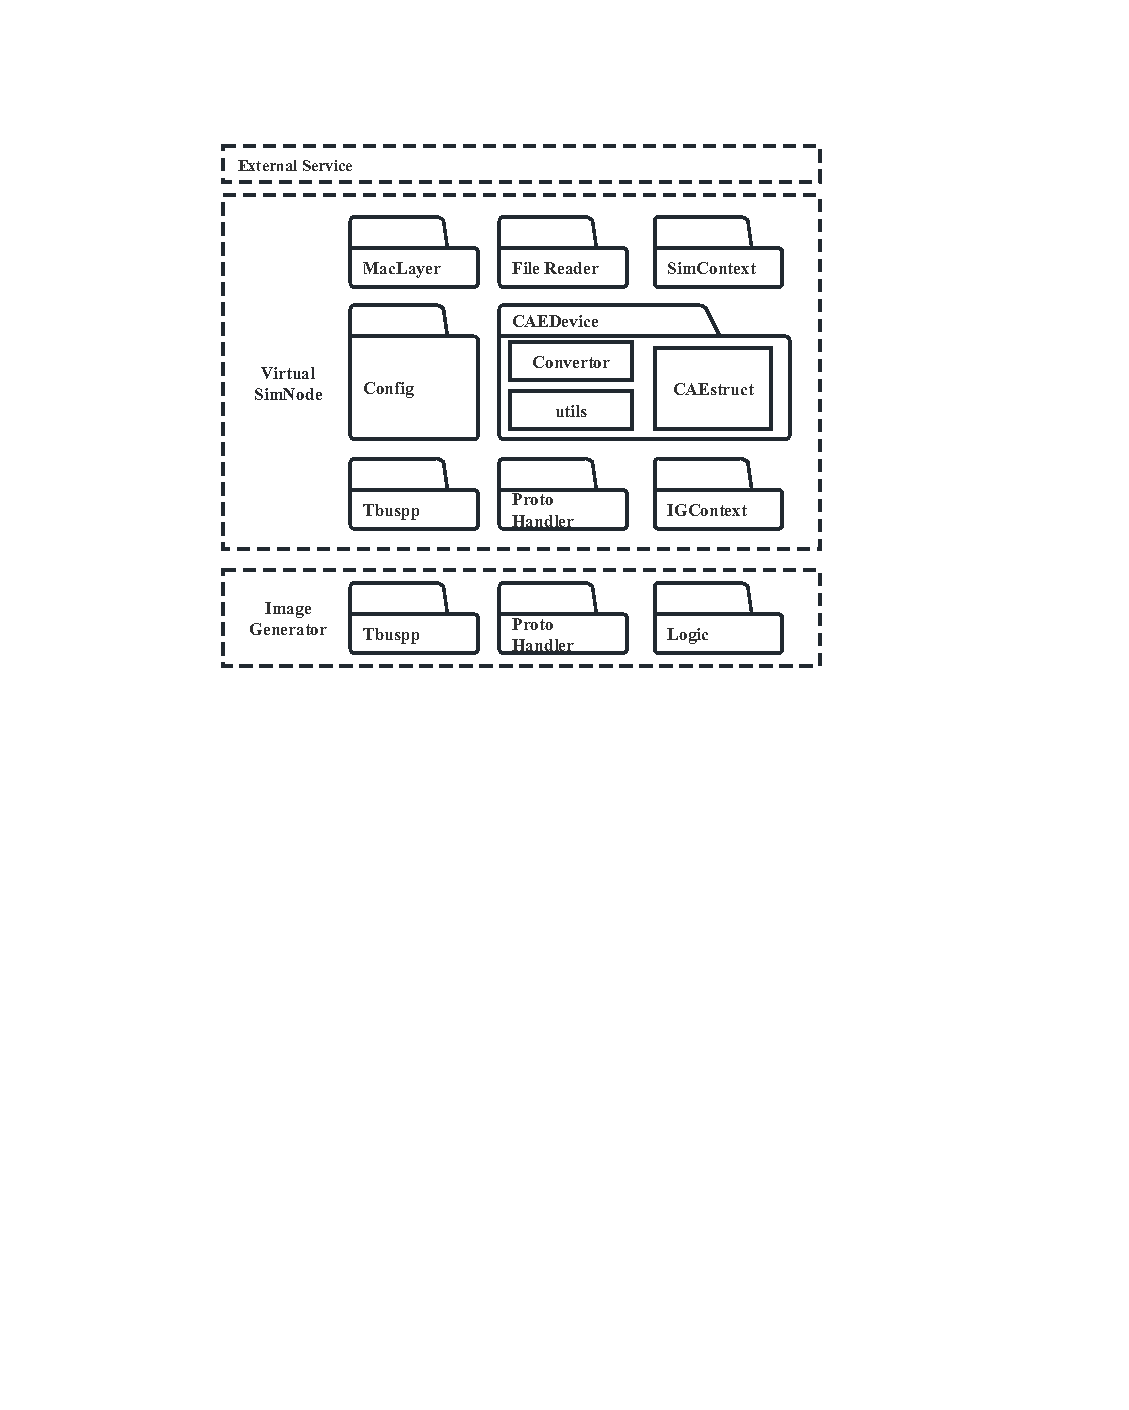
\includegraphics[width=0.7\textwidth]{pictures/devdiagram.pdf}
        \caption{开发视图}
        \label{dev}
    \end{center}
\end{figure}
\subsection{系统进程视图}
进程视图是用系统工程师的视角对系统进行阐述。可以详细阐述系统的动
态运行过程,重点描述系统运行时的行为。图\ref{procedure}是本系统的进程视图,
主进程启动时会先对各种交流环境初始化,对指令转换类进行注册,一切妥当后便可以接收来自仿真机的数据帧。收到消息后虚拟仿真机会立刻请求指令转换,生成自定义指令,发送给图像生成器进程。
图像生成器收到信息后立即对消息解封并反序列化,交付对应的逻辑处理。逻辑进程完成计算后可能会产生一些反馈指令,图像生成器将指令封装后反馈给虚拟仿真机,再请求转换为仿真机指令后便可发送给仿真机。
当然这之中逻辑线程的计算结果会提交给渲染进程完成画面生成,一般来讲逻辑进程比渲染进程快一帧。
\begin{figure}[h]
    \begin{center}
        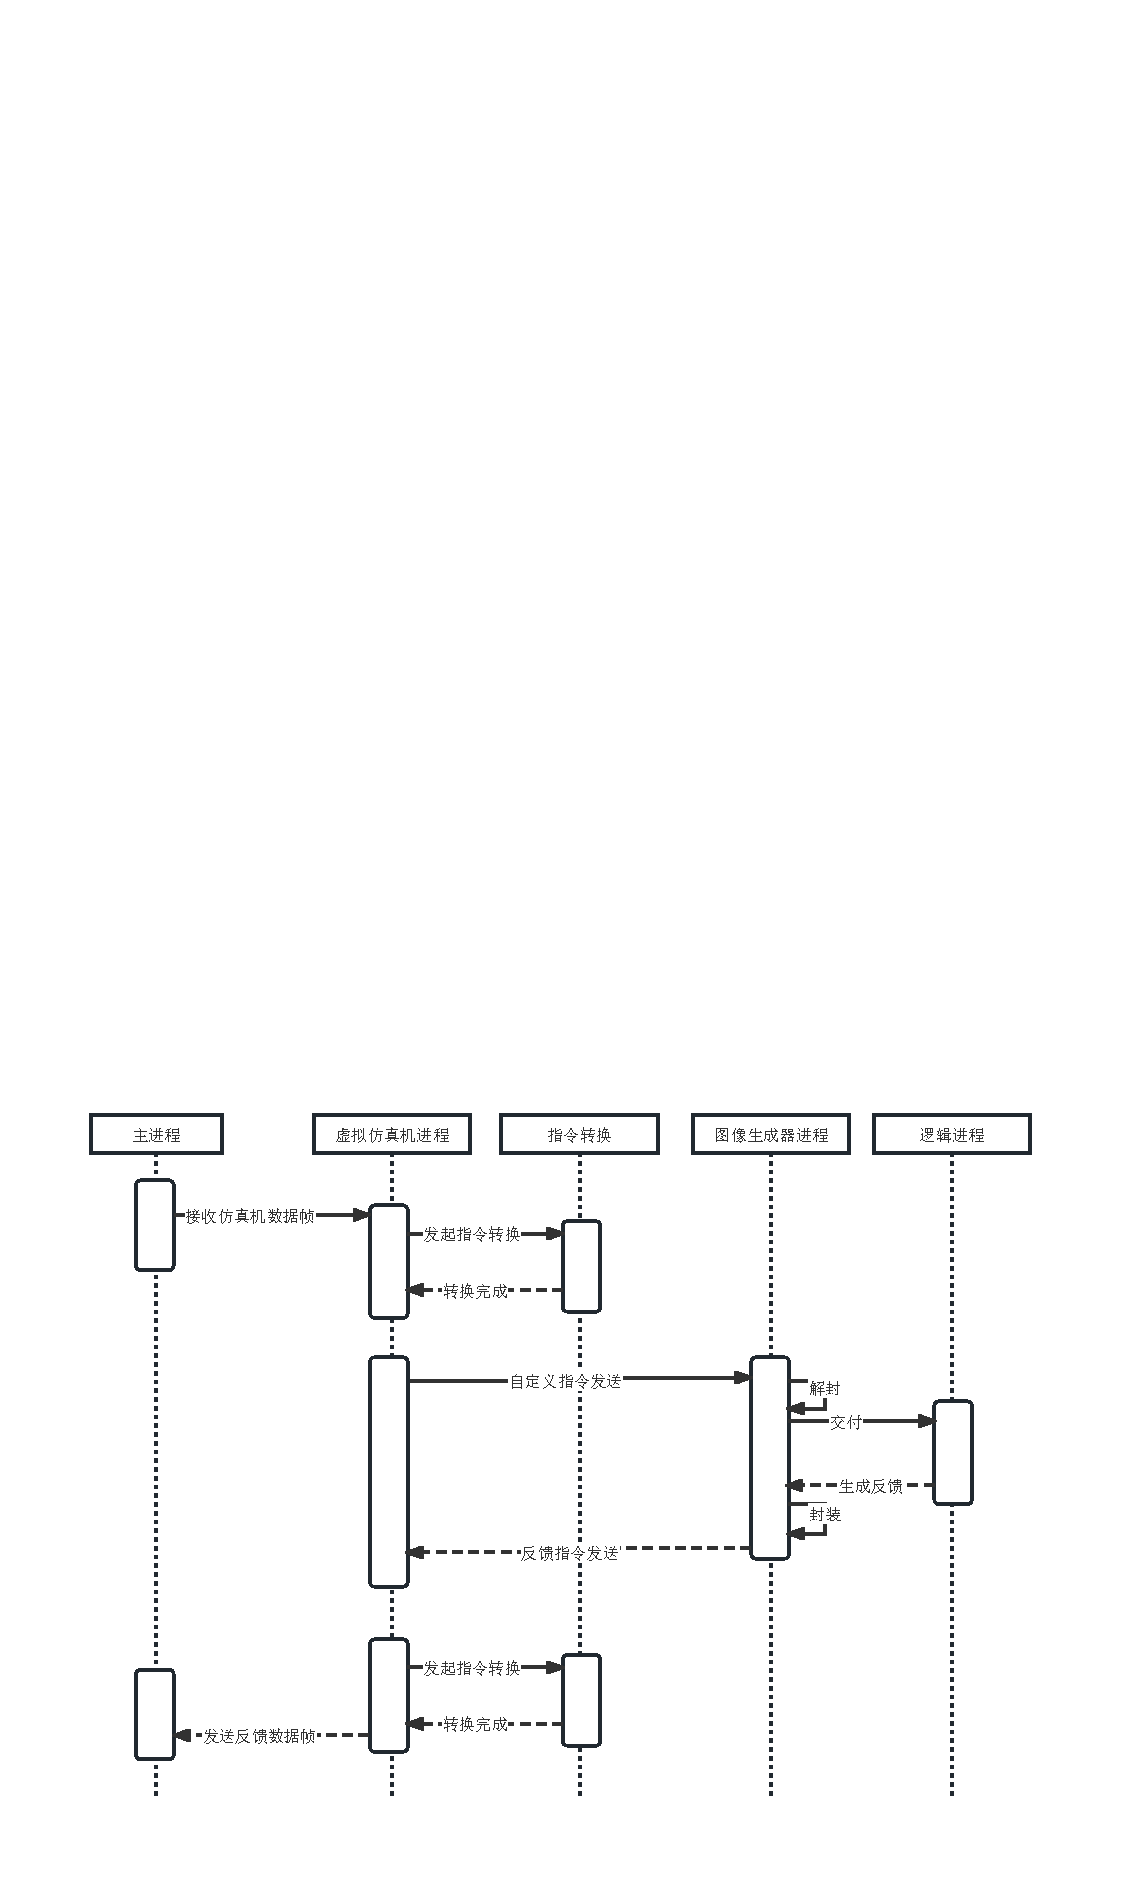
\includegraphics[width=\textwidth]{pictures/procedure.pdf}
        \caption{进程视图}
        \label{procedure}
    \end{center} 
\end{figure}
\subsection{系统部署视图}
部署视图是用运维人员的视角对系统进行阐释。它着重于解释说明系
统的整体物理结构和各组件之间的连接方式等,又称为物理视图。图\ref{deploydiagram}是本系
统的部署视图。飞行员在模拟座舱中操作被仿真机记录并进行仿真计算产生指令,通过以太网协议封装后发送给虚拟仿真机。指令的解析和转换在运行虚拟仿真机的机器内完成,通过TCP协议发送给图像生成器。图像生成器收到TCP消息后,根据解析的数据执行逻辑,完成场景的生成和渲染。
其产生的反馈信息会沿原路径回到仿真机。
\begin{figure}[h]
    \begin{center}
        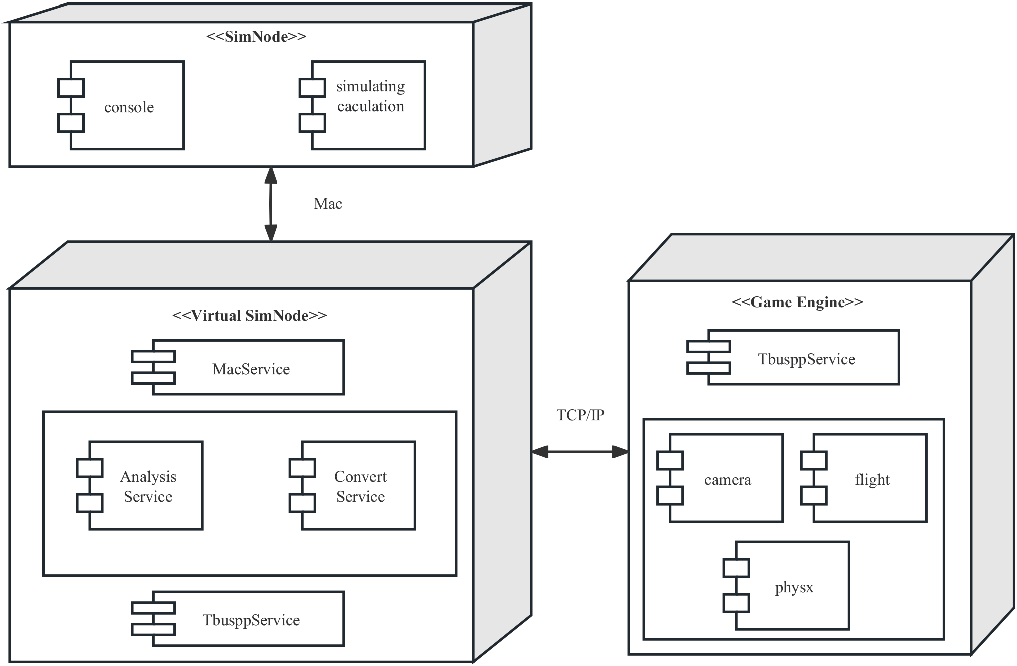
\includegraphics[width=0.8\textwidth]{pictures/deploydiagram.pdf}
        \caption{部署视图}
        \label{deploydiagram}
    \end{center}
\end{figure}

\section{本章小结}
本章开篇对于视景系统的工作方法做出说明。
根据说明可知本项目需要将视景系统接入一个不清楚接口的仿真机设备,于是通过结合文档和分析网络流量的方法解读出仿真机的交流协议。
明确了接入方法后,便可以按照软件开发的一般步骤进行。
首先,对数据交换子系统进行了需求分析,明确功能性需求和非功能性需求,
其次,通过用例图和用例描述表的形式给出场景说明。
最后,本章以系统开发4+1视图的形式给出了数据交换子系统的架构设计。
